\documentclass[type=bachelor]{thuthesis}
% 选项:
%   type=[bachelor|master|doctor|postdoctor], % 必选
%   secret,                                   % 可选
%   pifootnote,                               % 可选(建议打开)
%   openany|openright,                        % 可选,基本不用
%   arial,                                    % 可选,基本不用
%   arialtoc,                                 % 可选,基本不用
%   arialtitle                                % 可选,基本不用

% 所有其它可能用到的包都统一放到这里了,可以根据自己的实际添加或者删除。
\usepackage{thuthesis}

% 定义所有的图片文件在 figures 子目录下
\graphicspath{{figures/}}

% 可以在这里修改配置文件中的定义。导言区可以使用中文。
% \def\myname{薛瑞尼}

\begin{document}

%%% 封面部分
\frontmatter
\thusetup{
  %******************************
  % 注意:
  %   1. 配置里面不要出现空行
  %   2. 不需要的配置信息可以删除
  %******************************
  %
  %=====
  % 秘级
  %=====
  secretlevel={秘密},
  secretyear={10},
  %
  %=========
  % 中文信息
  %=========
  ctitle={基于浮动车轨迹数据的路况分析},
  cdegree={工学学士},
  cdepartment={计算机科学与技术系},
  cmajor={计算机科学与技术},
  cauthor={吴铮},
  csupervisor={向勇 副教授},
  %%cassosupervisor={陈文光教授}, % 副指导老师
  %%ccosupervisor={某某某教授}, % 联合指导老师
  % 日期自动使用当前时间,若需指定按如下方式修改:
  % cdate={超新星纪元},
  %
  % 博士后专有部分
  cfirstdiscipline={计算机科学与技术},
  cseconddiscipline={系统结构},
  postdoctordate={2009年7月——2011年7月},
  id={编号}, % 可以留空: id={},
  udc={UDC}, % 可以留空
  catalognumber={分类号}, % 可以留空
  %
  %=========
  % 英文信息
  %=========
  etitle={An Introduction to \LaTeX{} Thesis Template of Tsinghua University v\version},
  % 这块比较复杂,需要分情况讨论:
  % 1. 学术型硕士
  %    edegree:必须为Master of Arts或Master of Science(注意大小写)
  %             “哲学、文学、历史学、法学、教育学、艺术学门类,公共管理学科
  %              填写Master of Arts,其它填写Master of Science”
  %    emajor:“获得一级学科授权的学科填写一级学科名称,其它填写二级学科名称”
  % 2. 专业型硕士
  %    edegree:“填写专业学位英文名称全称”
  %    emajor:“工程硕士填写工程领域,其它专业学位不填写此项”
  % 3. 学术型博士
  %    edegree:Doctor of Philosophy(注意大小写)
  %    emajor:“获得一级学科授权的学科填写一级学科名称,其它填写二级学科名称”
  % 4. 专业型博士
  %    edegree:“填写专业学位英文名称全称”
  %    emajor:不填写此项
  edegree={Doctor of Engineering},
  emajor={Computer Science and Technology},
  eauthor={Xue Ruini},
  esupervisor={Professor Zheng Weimin},
  eassosupervisor={Chen Wenguang},
  % 日期自动生成,若需指定按如下方式修改:
  % edate={December, 2005}
  %
  % 关键词用“英文逗号”分割
  ckeywords={浮动车数据,低采样率数据 , 路口, 路况估计},
  ekeywords={Floating Car Data, Low Sampling Data, Road Junction,Traffic Situation Evaluation}
}

% 定义中英文摘要和关键字
\begin{cabstract}
随着出租车车载全球定位系统(GPS)装置的普及,浮动车(FCD)轨迹信息越来越容易获得。由于浮动车的轨迹信息有着非常好的城市覆盖率,而且数据量庞大,浮动车数据成为了城市交通路况计算中重要的数据来源。而高密度高准确度的GPS信息非常稀有,而且存储和传输成本高,这也使得研究低采样率的浮动车轨迹信息变得很有意义。

在本文中,我们讨论的是低采样率下的浮动车轨迹用于路况计算的情况,主要考虑了相邻两个数据点之间相隔一个路口的情况。本文中的模型采用线性回归作为主要方法,做了一些细节上的优化,在模拟环境下验证了方法的可行性。

  本文的创新点主要有:
  \begin{itemize}
    \item 低采样率下分析经过路口的浮动车轨迹
    \item 没有使用传统的平滑算法
  \end{itemize}

\end{cabstract}

% 如果习惯关键字跟在摘要文字后面,可以用直接命令来设置,如下:
% \ckeywords{浮动车数据,低采样率数据 , 路口, 路况估计}

\begin{eabstract}
With the popularity of taxi car global positioning system (GPS) devices, floating car data (FCD) is much easier to be obtained. As the trajectory of the floating car has a very good urban coverage and a large amount of data, floating car data has become an important source of data for urban traffic estimation. However, highly precise GPS traces are rarely available and brings a great pressure to both storage and transmission system hence it is meaningful to study the trajectory information of the floating car data with low sampling rate.

In this paper, We discuss the use of floating car data at low sampling rates for urban traffic situation evaluation taking the situation that adjacent two data points separated by an intersection into consideration. The model in this paper use linear regression as the main method and pay attention to the optimization of some details. We use simulation data to verify the feasibility of this method.

There are some points making our system different:
   \begin{itemize}
       \item Junction analysis of floating car data at low sampling rate
       \item Abandon the traditional smoothing algorithm
   \end{itemize}
   
\end{eabstract}

% \ekeywords{Floating Car Data, Low Sampling Data, Road Junction,Traffic Situation Evaluation}

% 如果使用授权说明扫描页,将可选参数中指定为扫描得到的 PDF 文件名,例如:
% \makecover[scan-auth.pdf]
\makecover

%% 目录
\tableofcontents

%% 符号对照表
\begin{denotation}[3cm]
\item[HPC] 高性能计算 (High Performance Computing)
\item[cluster] 集群
\item[Itanium] 安腾
\item[SMP] 对称多处理
\item[API] 应用程序编程接口
\item[PI] 聚酰亚胺
\item[MPI] 聚酰亚胺模型化合物,N-苯基邻苯酰亚胺
\item[PBI] 聚苯并咪唑
\item[MPBI] 聚苯并咪唑模型化合物,N-苯基苯并咪唑
\item[PY] 聚吡咙
\item[PMDA-BDA]	均苯四酸二酐与联苯四胺合成的聚吡咙薄膜
\item[$\Delta G$] 活化自由能 (Activation Free Energy)
\item[$\chi$] 传输系数 (Transmission Coefficient)
\item[$E$] 能量
\item[$m$] 质量
\item[$c$] 光速
\item[$P$] 概率
\item[$T$] 时间
\item[$v$] 速度
\item[劝学] 君子曰:学不可以已。青,取之于蓝,而青于蓝;冰,水为之,而寒于水。木
  直中绳。輮以为轮,其曲中规。虽有槁暴,不复挺者,輮使之然也。故木受绳则直,金就
  砺则利,君子博学而日参省乎己,则知明而行无过矣。吾尝终日而思矣,不如须臾之所学
  也;吾尝跂而望矣,不如登高之博见也。登高而招,臂非加长也,而见者远;顺风而呼,
  声非加疾也,而闻者彰。假舆马者,非利足也,而致千里;假舟楫者,非能水也,而绝江
  河,君子生非异也,善假于物也。积土成山,风雨兴焉;积水成渊,蛟龙生焉;积善成德,
  而神明自得,圣心备焉。故不积跬步,无以至千里;不积小流,无以成江海。骐骥一跃,
  不能十步;驽马十驾,功在不舍。锲而舍之,朽木不折;锲而不舍,金石可镂。蚓无爪牙
  之利,筋骨之强,上食埃土,下饮黄泉,用心一也。蟹六跪而二螯,非蛇鳝之穴无可寄托
  者,用心躁也。—— 荀况
\end{denotation}



%%% 正文部分
\mainmatter
\chapter{引言}
\label{chp1}

\section{背景}

随着经济发展,汽车的普及率越来越高,已经成为了是人们最常选择的出行手段之一。而汽车持有率的增加导致了很多交通问题,这也就使得实时路况计算变得十分重要。实时路况计算依赖可靠的实时道路轨迹数据,对于高速公路等简单结构的区域,一般采用固定探测装置来进行路况采集~\cite{yuan2014network,wang2005real}。而对于相对复杂的城市区域,装有GPS(Global Position System)系统的浮动车是最近几年兴起的道路路况计算很好的数据来源。与传统的固定探测装置相比,浮动车不仅部署起来更简单,而且在城市区域拥有非常好的覆盖率,部署的成本也更低。但是高采样率的浮动车轨迹数据很难获得,而且储存和传输成本过高,所以我们主要研究低采样率浮动车轨迹数据下的路况计算~\cite{rahmani2010requirements,brockfeld2007benefits}。

对于复杂的城市区域道路网络来说,各个路段的交叉口是对交通状况产生影响最重要的因素之一,判定路口行驶状况的参数有等待队列长度,车辆停止率等等。在本文中,我们忽略了车辆经过路口时的行驶细节,将信号灯或者其他类似于立交桥的道路切换系统中花费的时间统一计作一个虚拟的路口转向延迟。这样做的好处是可以忽略路口的实际结构,使得模型的可扩展性变得更强。

在我们遇到的实际浮动车轨迹数据中,低采样率的数据(两个相邻点之间相隔超过30秒)占到全部数据中的大多数~\cite{yue2009urban},而且95\%以上的数据相邻两个点之间至少间隔了一个路口,这也就使得研究使用跨路口的低采样率浮动车轨迹数据判断两段路分别路况的算法变得很有意义。

\section{研究目标}

由于城市路段路口之间的间隔较短,使得车辆花费在路口的等待时间占到了很大比例,使得使用传统的路况估计方法得到的结果会和实际结果有着比较大的偏差,所以我们需要设计一个模型和算法估计城市区域路口的转向延迟,使得数据的利用率变高,结果也更接近实际值,提高整个城市路况估计系统的准确度。

\section{文章结构}

根据本文的内容,文章一共分成5个章节:
\begin{itemize}

\item 第一章是引言,主要介绍了论文的背景和目标。
\item 第二章是综述,具体介绍了论文想要处理的问题和相关的工作。
\item 第三章是算法设计,介绍了模型的建立和算法的选择。
\item 第四章是实验,介绍了实验的设计和结果分析。
\item 第五章是结论,总结了算法的优势和不足,以及今后可能的优化方向。

\end{itemize}
\chapter{综述}
\label{chap2}

\section{问题综述}
在计算路况时,由于数据的稀疏性,会出现两个GPS坐标之间相隔一个路口甚至更多的情况,但是我们要分别统计每一段路的路况,所以要把两段道路的路况进行分离。建立模型时把每段轨迹的时间分成两段路的用时加上虚拟的路口转向延迟三个部分,对于每个路段,如果存在正反两个方向则两个方向的路况互不干扰单独计算。

拿十字路口举例,如图~\ref{fig:1}所示,一个路口的参数包含4个路段每个路段两个方向共8个方向的路况参数,路口12个方向的转向延迟。当前系统的处理方式是直接把每段轨迹的时间按照经过道路的长度加权分配在每段路上,再由通过同一路段的所有轨迹加权得到该路段的用时,推算出平均速度来表示路况。

\begin{figure}[H] 
  \centering
  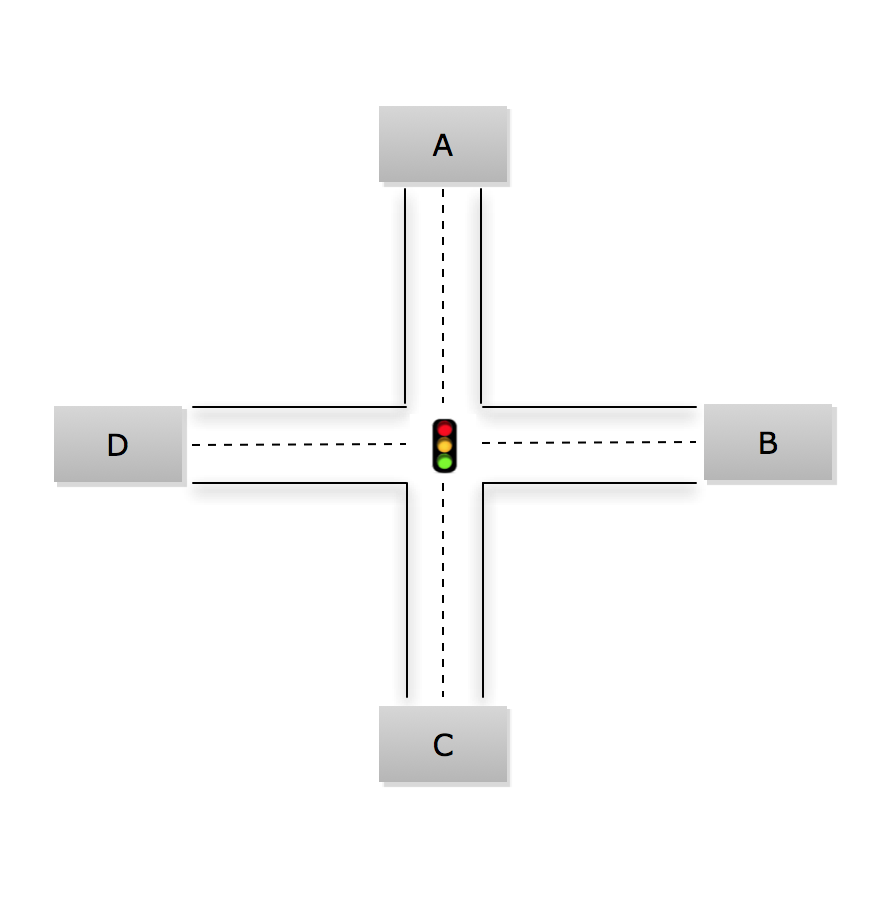
\includegraphics[width=3.5in]{intersection}
  \caption{路口示意图}
  \label{fig:1}
\end{figure}

拿AB段举例,将路口设为O点,这时如果出现AO段行驶畅通而OB段堵塞的情况,时间会平摊到AO和OB两段,这样计算出的结果不能反映真实的路况。又考虑到一定时间内路况不出现大的变化,本文的算法选取一定时间内通过同一路口的数据,使用这些数据直接计算出每一段的精确路况,从而能够更准确地反映每段路分别的路况信息。


\section{相关工作}
\label{sec:related_work}

\subsection{平滑算法}

\begin{figure}[H] 
  \centering
  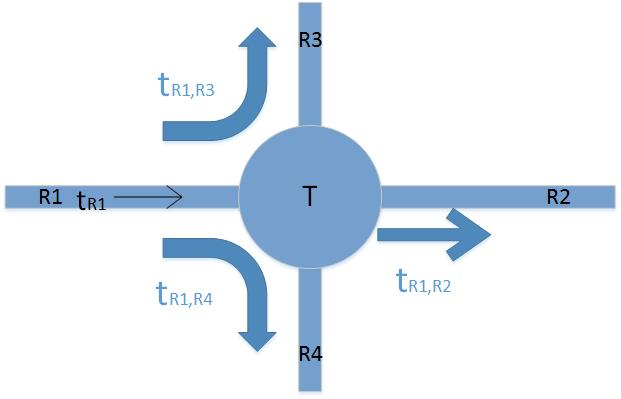
\includegraphics[width=3in]{road_model}
  \caption{平滑算法}
  \label{fig:2}
\end{figure}

该算法中跨路口的轨迹,如图~\ref{fig:2}所示,拿$R1\to R2$举例,包括前一段路R1的行驶时间$t_{R1}$,转向延迟$t_{R1,R2}$和第二段路的行驶时间$t_{R2}$(\ref{f2.1.1})。然后计算当前道路的通过时间以及到下一条道路的转向时间的和在总时间中的比重(\ref{f2.1.2})。之后计算实际花费的时间(\ref{f2.1.3})。最后按比例分配行驶时间与转向时间(\ref{f2.1.4})。这种做法优势是实现起来非常简单,通用性强,但是对于某些路况分布不均匀情况可能效果不是很理想。

\begin{equation}
t=t_{R1}+t_{R1,R2}+t_{R2}
\label{f2.1.1}
\end{equation}
\begin{equation}
percentage = (cover\_rate\times road\_length/road\_speed + turn\_time) / total\_time;
\label{f2.1.2}
\end{equation}
\begin{equation}
real\_time = interval\times percentage;
\label{f2.1.3}
\end{equation}
\begin{equation}
turn\_delay = real\_time \times turn\_time/(turn\_time + trip\_time);
\label{f2.1.4}
\end{equation}

\subsection{路段分解算法}

\begin{figure}[H] 
  \centering
  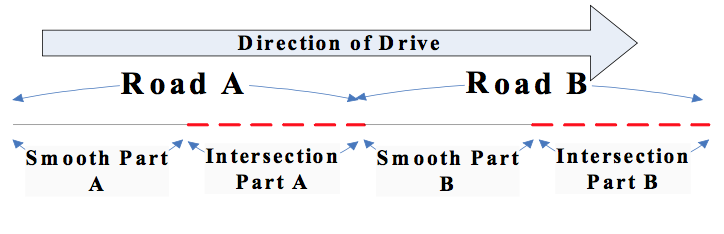
\includegraphics[width=3in]{road_separation}
  \caption{路段分解算法}
  \label{fig:3}
\end{figure}

算法引用自Yue发表在ICCTP 2009的一篇论文中~\cite{yue2009urban}。该算法将道路分成平滑部分(Smooth Part)和路口部分(Intersection Part)。 IP段长度由路由确定,是由道路等级和历史等待队列长度计算得出的。还将两条相邻的路段定义为道路A和道路B,表示为$R_{}A$和$R_{B}$。两个连续的GPS信号分别被定义为$G_{j}(x_{j},y_{j},T_{j})$和$G_{j + 1}(x_{j + 1},y_{j + 1},T_{j + 1})$,其中(x,y)分别是匹配的GPS坐标,而T是相应的时间戳。计算$R_{A}$段行驶速度的公式如下(\ref{f2.2.1})。

\begin{equation}
TS_{A}=\frac{L_{TotalA}}{\frac{L_{intersection}}{TS_{intersection}^{A}}+\frac{L_{TotalA}-L_{intersection}}{TS_{SP}^{A}}}
\label{f2.2.1}
\end{equation}

其中,$TS_{A}$代表道路A的平均速度,分母左右分别为路口路段的时间和平滑路段的时间。$TS_{SP}^{A}$伪平滑路段的速度,使用所有在平滑路段A上前后两殿的平均速度按所占道路比例加权,找不到这样的点则使用该段的瞬时速度代替。$TS_{intersection}^{A}$则是路口路段的速度,使用路口路段车辆平均瞬时速度来计算。这种算法十分依赖瞬时速度,然而我们得到的浮动车GPS数据的瞬时速度经常出现非常大的偏差,所以这种算法也不适合我们的系统。

\subsection{延迟估计算法}

\begin{figure}[H] 
  \centering
  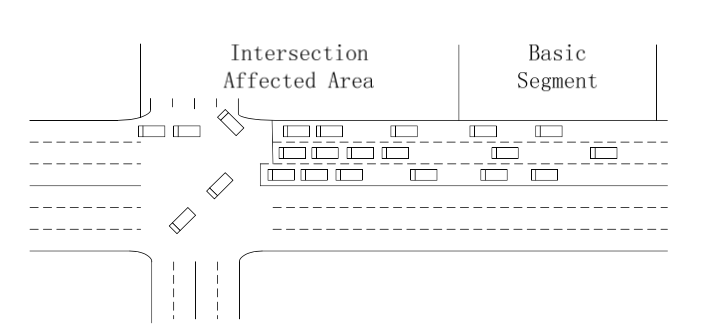
\includegraphics[width=3in]{delay}
  \caption{延迟估计算法}
  \label{fig:4}
\end{figure}

算法引用自Zhao-cheng2014年发表在CICTP的一篇论文中~\cite{he2014delay}。算法的原理是确定路口受影响区域外的两个最近的GPS点,来确定路口行驶时间。在计算路口延迟之前,需要车辆在路口的行驶时间$T_{fcd}$和车辆在加速行驶速度$T_{exp}$的行驶时间。文章中直接采用道路设计速度作为车辆的快速行驶速度。

\begin{figure}[H] 
  \centering
  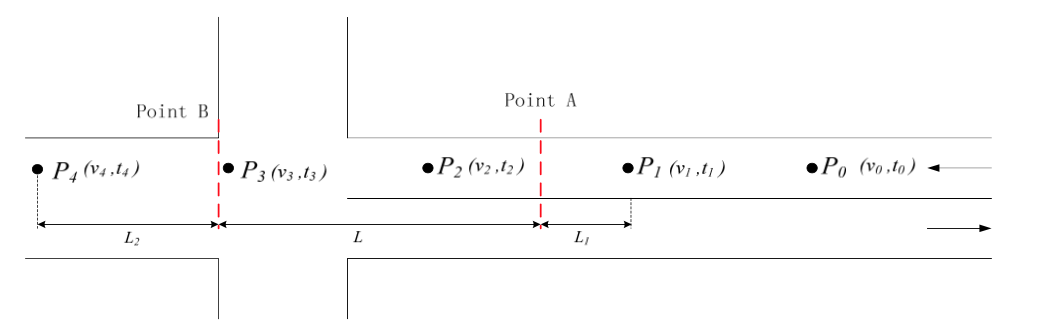
\includegraphics[width=3in]{delay2}
  \caption{计算原理}
  \label{fig:5}
\end{figure}

算法的计算原理见图~\ref{fig:5},其中点A和点B之间的区域是路口影响区域。 假设一个跨越十字路口的出租车轨迹包括几个GPS点$(P_{1},P_{2} ...)$。 选择路口影响区域外的两个最近点(即图~\ref{fig:5}中的$P_{1}$,$P_{4}$)。这两点的速度需要大于零。 点$P_{1}$用于估计进入路口影响区域的车辆的时间戳。 $P_{4}$点则用于估计离开路口影响区域的车辆的时间戳。可以得出如下的公式:

\begin{equation}
t_{A}=t_{1}+\frac{L_{1}}{v_{1}}
\end{equation}

\begin{equation}
t_{B}=t_{4}+\frac{L_{2}}{v_{4}}
\end{equation}

\begin{equation}
T_{fcd}=t_{B}-t_{A}= \left( t_{4}+\frac{L_{2}}{v_{4}}\right) - \left( t_{1}+\frac{L_{1}}{v_{1}}\right)
\end{equation}

参数$v_{1}$,$v_{4}$,$t_{1}$,$t_{4}$是已知的,可以直接通过GPS数据获得。 点$P_{1} $和$P_{4}$的位置可以通过上面的映射对应算法得出。之后就可以计算$L_{1}$,$L_{2}$。 因此,延迟估计的公式如下:

\begin{equation}
D = T_{fcd} - T_{exp} = t_{B} - t_{A} - \frac{L}{v_{exp}}
= \left( t_{4}+\frac{L_{2}}{v_{4}}\right) - \left( t_{1}+\frac{L_{1}}{v_{1}}\right) - \frac{L}{v_{exp}}
\end{equation}

该算法的优势是对于路口的判断很精确,但是需求的数据密度还是相对比较多,需要数据间隔在30s左右,但是我们的数据不能达到这种要求,间隔基本在60s左右,所以这种算法还是无法适用于我们当前的系统。


\chapter{算法设计}
\label{chap3}

\section{算法描述}

\subsection{设计思路}

前面提到现有的算法如果跨路口的两段路出现一段堵车而另一段通行良好的情况,时间会平摊到两段,不够准确。由于算法要求在线,但历史数据可以从服务器端取得,考虑5分钟内路况通常不会出现大的变化,当新的轨迹数据进入系统后,我们可以利用过去五分钟内的历史数据来计算出该轨迹经过路段的准确路况,也保证了算法的在线性。

\subsection{算法优势}

相对于平滑算法,我们对于轨迹数据的利用率更高,能够在相邻道路间速度差异较大时得到比较理想的结果,实现起来也较为简单,算法的复杂度不高,可能很快地计算出结果,能够适应在线系统的要求。模型同样具有可扩展性,只需要简单修改就可以应对多叉路口或者立交桥等复杂路口的情况,也可能扩展到跨越多个路口的情况。

\section{具体实现}

\subsection{模型建立}

\begin{figure}[H] 
  \centering
  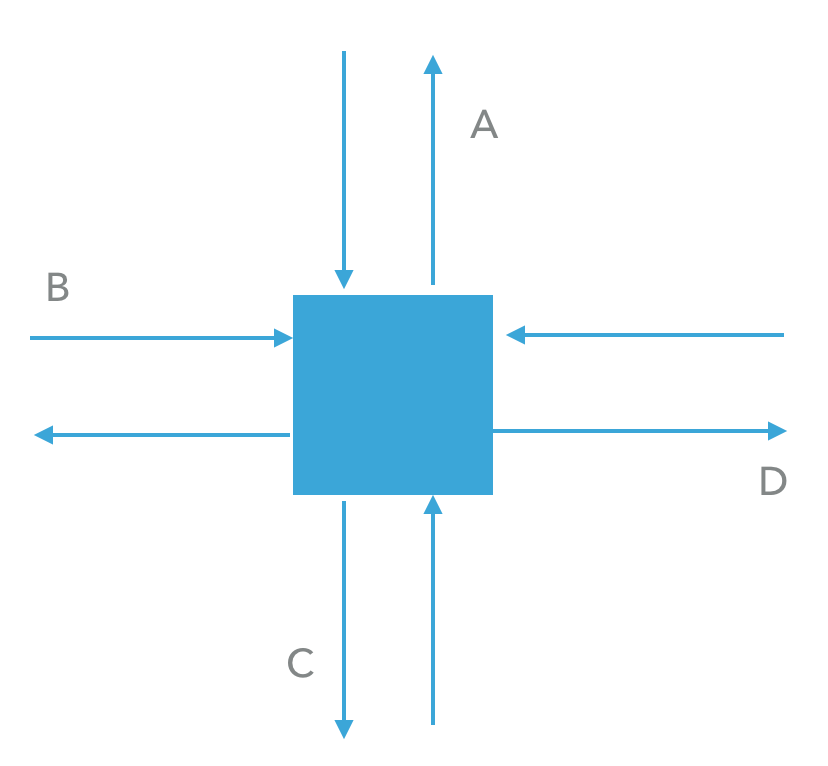
\includegraphics[width=3in]{model_bulid}
  \caption{模型示意图}
  \label{fig:3.1}
\end{figure}

如图\ref{fig:3.1}所示,我们将路口部分抽象成一个黑盒,一个十字路口就被抽象成A,B,C,D4段路径正反8个方向和黑盒中连接这8个方向的12组转向延迟。假设进入十字路口的路段为A1,B1,C1,D1,离开十字路口的则为A2,B2,C2,D2。路口的轨迹数据信息就被抽象成了12组方程。

\begin{equation}
k1_{A1,B2} \times T_{A1} + k2_{A1,B2} \times T_{B2} + turn_{A1,B2} = t_{1}
\end{equation}

\begin{equation*}
k1_{A1,C2} \times T_{A1} + k2_{A1,C2} \times T_{C2} + turn_{A1,C2} = t_{2}
\end{equation*}

......

\begin{equation*}
k1_{D1,C2} \times T_{D1} + k2_{D1,C2} \times T_{C2} + turn_{D1,C2} = t_{12}
\end{equation*}

其中k1与k2是指轨迹覆盖到当前路段的百分比,turn是指该方向的转向延迟,包含花费在交通信号灯或者路口切换装置上的时间,把这些时间加在一起抽象成一个转向延迟的概念。

\subsection{单方向算法}

得到5分钟内的轨迹数据后按照12个方向进行划分,选取出轨迹数量最多的方向先入手。假设该方向5分钟内有n条轨迹,则我们可以得到n组方程,如下所示。再对方程组做线性回归求出拟合直线,之后利用直线的斜率和截距信息计算出花费在第一条路的时间$T_{1}$,花费在第二条路的时间$T_{2}$以及转向延迟turn。

\begin{equation}
\begin{bmatrix}
k_{11}  &  k_{21}   &1\\
k_{12}  &  k_{22}   &1\\
 \vdots   & \vdots   & \vdots  \\
k_{1n}  & k_{2n}    &1\\
\end{bmatrix} \times 
\begin{bmatrix}
T_{1}  \\
T_{2}  \\
turn \\
\end{bmatrix} = 
\begin{bmatrix}
t_{1}  \\
t_{2}  \\
\vdots \\ 
t_{n} \\
\end{bmatrix}
\end{equation}

\subsection{线性回归}
如果数据量多于3条,那么方程是无解的,所以我们需要引入线性回归的算法来近似地得出每段路的路况结果。把总时间$t_{i}$看成随机变量y,把每条道路的通行时间看成自变量$x_{i}$,就有(\ref{f3.1})。

\begin{equation}
y_{i} = \theta^{T}x_{i}+ \epsilon_{i}
\label{f3.1}
\end{equation}

这时使用最小二乘法求出一条使得所有点到拟合直线垂直距离平方之和(\ref{f3.2})最小的拟合直线。

\begin{equation}
\frac{1}{2} \sum_{i=1}^{n} (h_{\theta} (y_{i}-x_{i}))^{2}
\label{f3.2}
\end{equation}

使用最小二乘法对轨迹数据做线性回归也就相当于做了一个最大似然估计,而类似的还有一种方法是使用贝叶斯方法来对轨迹数据做线性回归。Bayes方法的关键是计算后验概率,已知先验分布$p(\theta )= N(0,\tau^{2}I)$之后,我们使用bayes公式得到(\ref{f3.3})

\begin{equation}
p(\theta |S) = \frac{p(S|\theta )p(\theta )}{p(S)} 
\label{f3.3}
\end{equation}

之后以$\theta$为底做积分可以得到y在当前的数据样本空间下的分布(\ref{f3.4}),再对y积分得到线性回归的预测期望值(\ref{f3.5})

\begin{equation}
p(y|x,S)=\int_{\theta}p(y|x,\theta )p(\theta |S)d\theta
\label{f3.4}
\end{equation}

\begin{equation}
E[y|x,S]=\int_{y}p(y|x,S)ydy
\label{f3.5}
\end{equation}

Bayes方法和前面普通的最小二乘法做线性回归最大的区别就是加入了$\theta$的先验概率,也就是要找到使得(\ref{f3.6})最小的拟合直线作为结果。

\begin{equation}
\frac{1}{2} \sum_{i=1}^{n} (h_{\theta} (y_{i}-x_{i}))^{2} + \frac{\theta ^{2}}{2\tau ^{2}}
\label{f3.6}
\end{equation}

bayes方法对比最小二乘法最大的优势就是加入一个先验概率来在一定程度上规避掉过拟合的情况,在图\ref{fig:3.2}中我们选取了一些模拟数据加入了随机的噪声,对比最小二乘法和Bayes方法的效果。

\begin{figure}[H] 
  \centering
  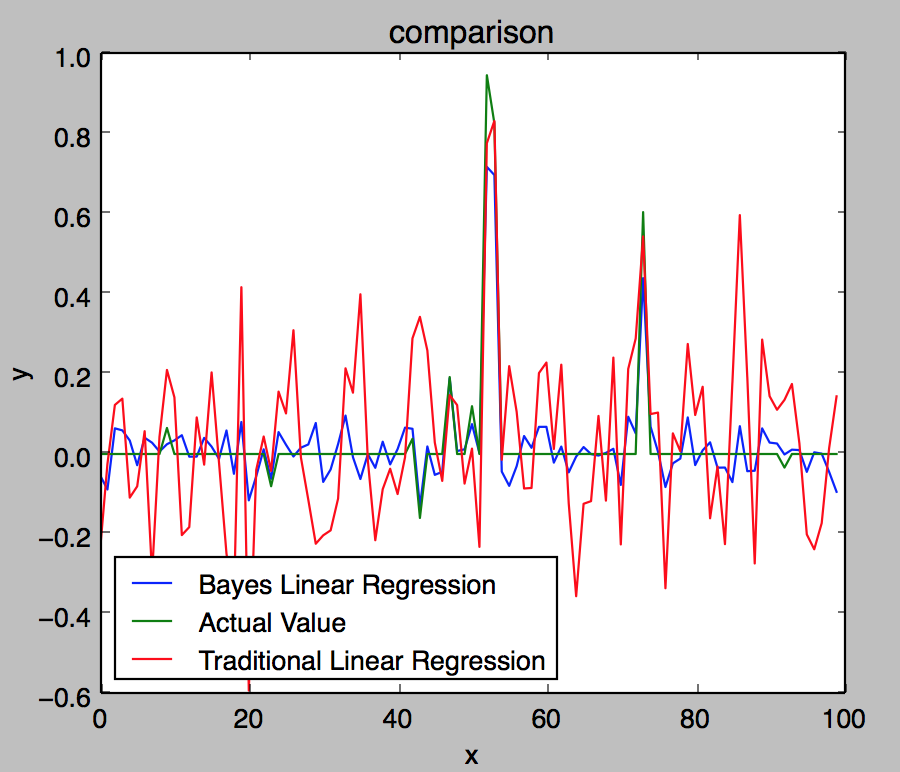
\includegraphics[width=3in]{comparison}
  \caption{Bayes对比最小二乘法}
  \label{fig:3.2}
\end{figure}

图\ref{fig:3.2}中绿色为原始数据,蓝色为Bayes方法回归结果,红色为最小二乘法的回归结果。我们可以看出总体上相比于最小二乘法,Bayes方法回归出的结果更接近于实际值,但是在实际数据中随着数据量的增加,最小二乘法的精确度会比Bayes方法更高,所以我们决定视数据量多少混合使用这两种算法进行计算,具体的结果会在第4章实验部分展示。

\subsection{多方向混合的算法}

考虑通过同一路段的三个方向的轨迹,其中有一条为右转的轨迹,而右转方向通常不需要等待信号灯,结果较为准确,需要的轨迹数量更少,如果可以找到右转的轨迹则先使用右转的轨迹计算得出该路段的路况,之后再结合另外两个方向的轨迹信息求解另外两个方向的路况信息。

对于路口整体的轨迹数据,我们使用相对方向直行和左转一般同时放行,得出相对方向直行和左转的红绿灯周期相同,所以转向延迟相近,计算出到一个方向的路况信息之后可以将转向延迟应用于其对应方向的路况计算,减少数据的需求量,综合这些信息我们设计了一个系统来对路口整体路况做计算,流程图如图\ref{fig:3.3}。

\begin{figure}[H] 
  \centering
  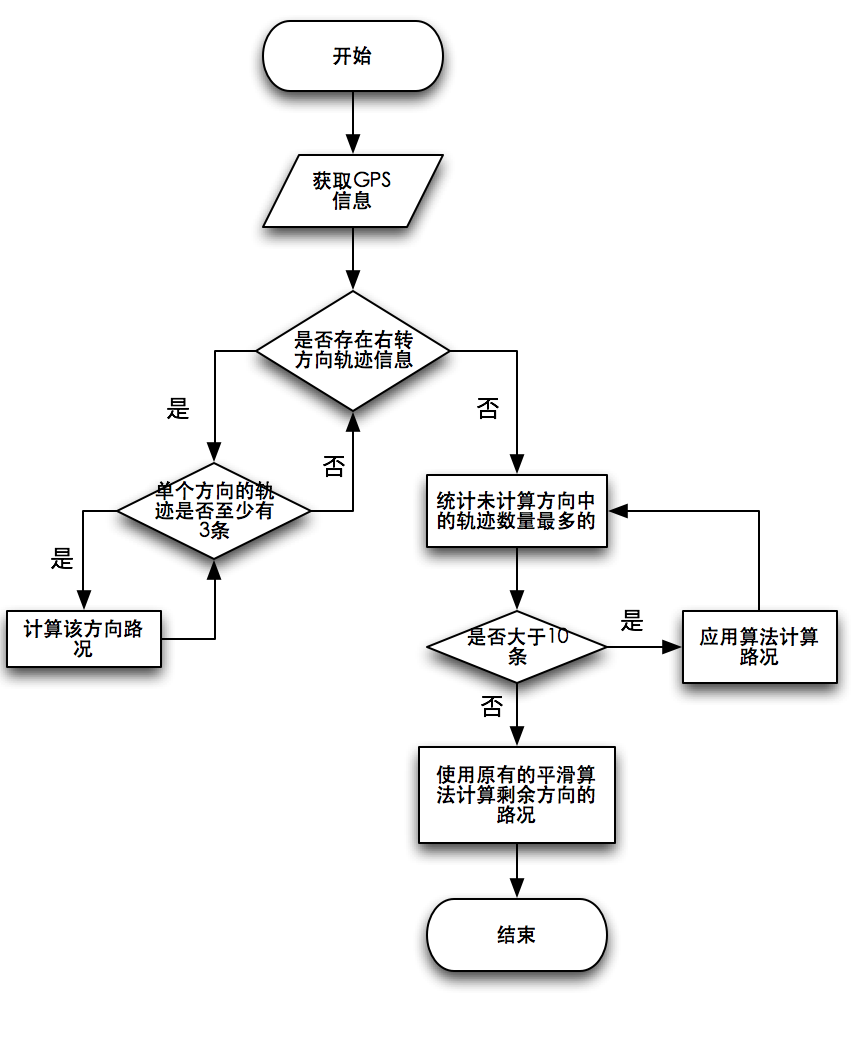
\includegraphics[width=3in]{flowchart}
  \caption{流程图}
  \label{fig:3.3}
\end{figure}

\section{细节改进}

\subsection{细化路口延迟}
为了细化车辆在路口的转向延迟,我们设计了一个方法来计算车辆在路口的等待队列长度,使用静止点序列$A_{n}$的平均值的2倍和和该序列的最大值来估计等待队列长度。
\begin{equation}
waiting\_queue = \max (A_{i}|i=1,2...n,2\times average(A_{n}))
\label{f3.7}
\end{equation}

之后我们细化了路口的转向延迟T(\ref{f3.8})
\begin{equation}
T = t_{2}-t_{1}-|p_{1}-j_{1}|/v_{1}
\label{f3.8}
\end{equation}
其中T为路口延迟,$t_{2}$和$t_{1}$分别是转弯过程中起始和终止点的时间戳,而$|p_{1}-j_{1}|$表示路口等待队列的长度,$v_{1}$是前一段路平滑路段的平均速度。

\subsection{排除异常点}

由于行驶轨迹数据带有一定的随机性,可能出现驾驶员异常操作或道路匹配错误等原因产生的异常数据,所以我们需要将数据中的异常点排除。对于自变量y和拟合向量$\hat{y} = Py$,我们可以得到残差向量$e = y - \hat{y} = (1-P)y$,计算残差平方和$RSS=e^{T}e$进而我们将残差标准化(\ref{f3.12})其中$\hat{\sigma} $为残差的参照值(\ref{f3.11}),假设数据满足正态分布为$N(0,1)$的随机样本,那么$r_{i}$落在$[-2,2]$的概率$P(\mu - 2\sigma < U < (\mu + 2\sigma ) = 95\%$,所以如果$|r_{i}|>2$那么这个点就被视为异常点,将其删除。如图\ref{fig:3.4},该图为一组左转数据的残差图,对于红色的两个点,我们在计算时将其删除,避免对整体结果产生偏差。

\begin{equation}
\hat{\sigma}=\sqrt{RSS/(n-k-1)}
\label{f3.11}
\end{equation}

\begin{equation}
r_{i} = \frac{e_{i}}{\hat{\sigma}\sqrt{1-p_{ii}}}, i = 1,2,...,n
\label{f3.12}
\end{equation}

\begin{figure}[H] 
  \centering
  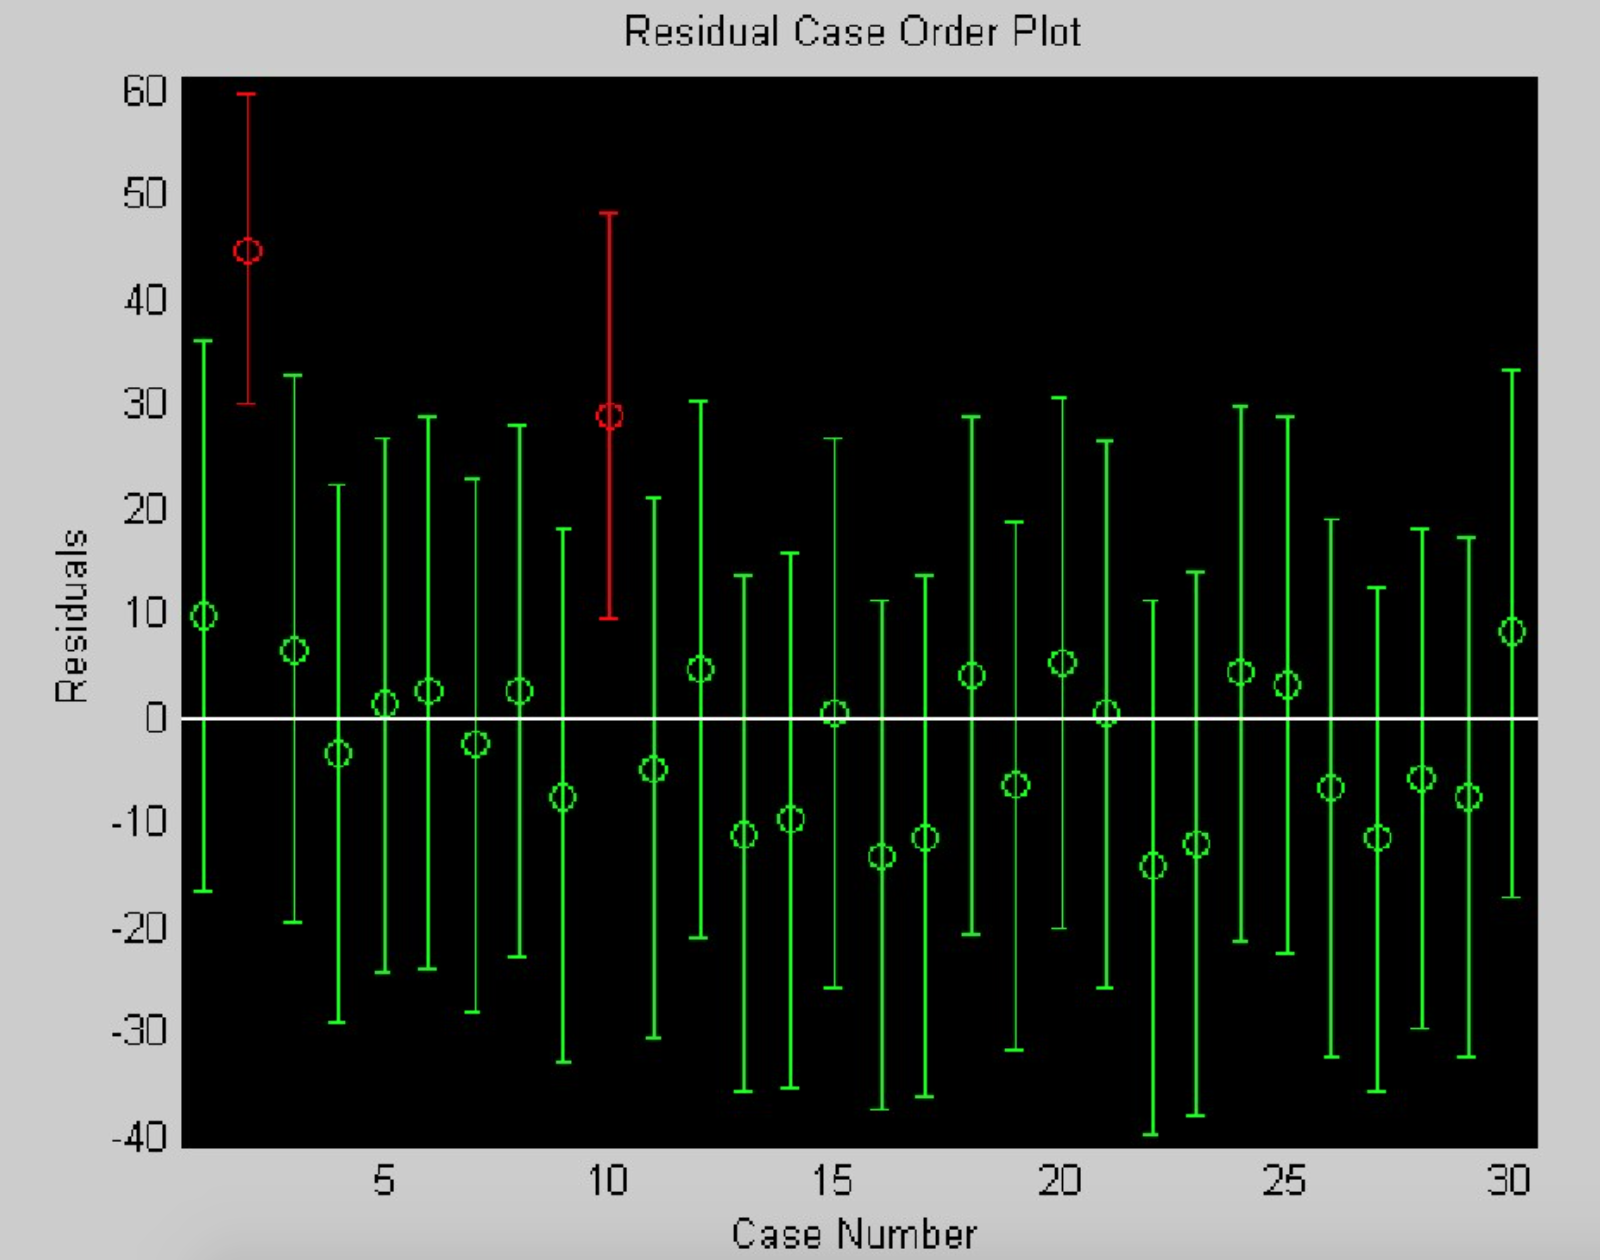
\includegraphics[width=3in]{residual}
  \caption{残差图}
  \label{fig:3.4}
\end{figure}

\subsection{回归方程式变形}
由于有的时候GPS轨迹信息的采样间隔不变,比如有些数据固定隔60s取一个点,直接\ref{f3.9}对采用线性回归的方法由于$T_{total}$不变不能得到满意的效果,所以要对式子进行变形\ref{f3.10}。这样做可以得到两段路的行驶时间,但是只能将路口延迟近似为一个既得的固定值,会对计算的精度造成影响,所以在GPS轨迹信息间隔不固定时还是采用原有的\ref{f3.9}。
\begin{equation}
k_{1} \times T_{1} + k_{2} \times T_{2} + T_{turn} = T_{total}
\label{f3.9}
\end{equation}

\begin{equation}
T_{1} + \frac{k_{2}}{k_{1}} \times T_{2}  = \frac{T_{total} - T_{turn}}{k_{1}}
\label{f3.10}
\end{equation}
\chapter{实验}
\label{chap4}

\section{实验设计}

本文中使用sumo作为仿真实验工具,生成模拟道路和信号灯,并且在地图上随机生成车辆获取车辆的轨迹信息来进行仿真试验。参数的设置为每段路的长度为1500m,车辆限速初始为90km\textbackslash h,实验过程中会视情况调整,一个交通信号灯的周期为140s,其中每个方向直行放行40s之后左转放行30s,右转方向为全时绿灯的状态。

\begin{figure}[H] 
  \centering
  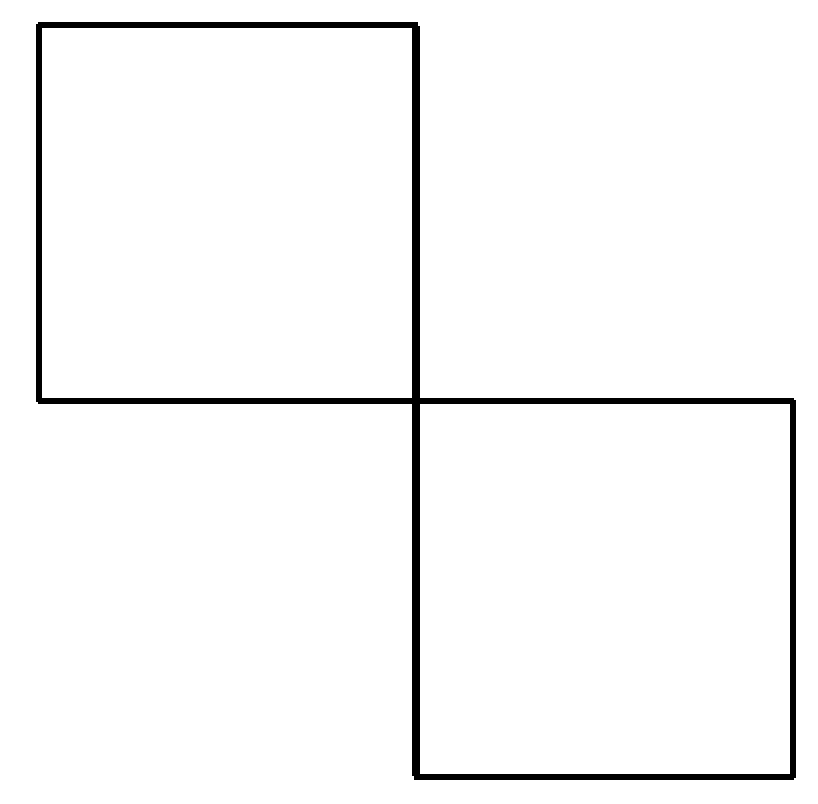
\includegraphics[width=2.5in]{simulation}
  \caption{地图}
  \label{fig:4.1}
\end{figure}

为了让轨迹数据能够集中通过十字路口,主要地图设计成如图\ref{fig:4.1},为一个"8"字形地图,使得随机的车辆能够在地图中随意行驶并且集中地通过中心的路口。

\begin{figure}[H] 
  \centering
  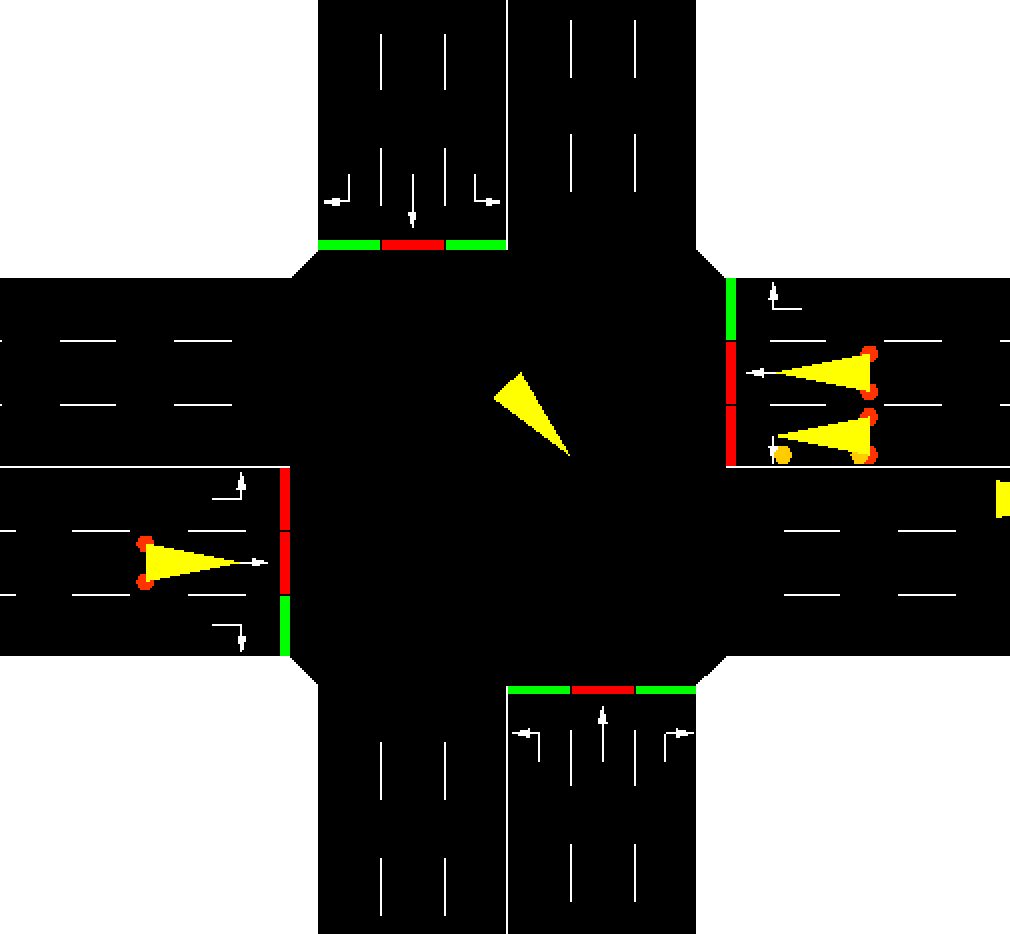
\includegraphics[width=3in]{cross}
  \caption{路口放大}
  \label{fig:4.2}
\end{figure}

模拟过程可以通过sumo-gui直观地看到,可以观察每辆车的具体行驶轨迹,路口模拟效果如图\ref{fig:4.2},可以清晰地看到每辆车和红绿灯的状态。

\section{实验结果分析}

\subsection{对比Bayes和最小二乘法}
从图\ref{fig:4.8}中我们可以看到,Bayes方法在数据量较少的时候更加稳定,准确度也比最小二乘法更高,最小二乘法等价于最大似然估计,在数据量小的时候会出现过拟合的现象,但是随着数据量逐渐增加准确度会超过Bayes方法,所以我们会在数据量较少(少于14组时)使用Bayes方法拟合,在数据量较多的时候使用最小二乘法进行更精确的估计,将两种算法结合到一起。

\begin{figure}[H] 
  \centering
  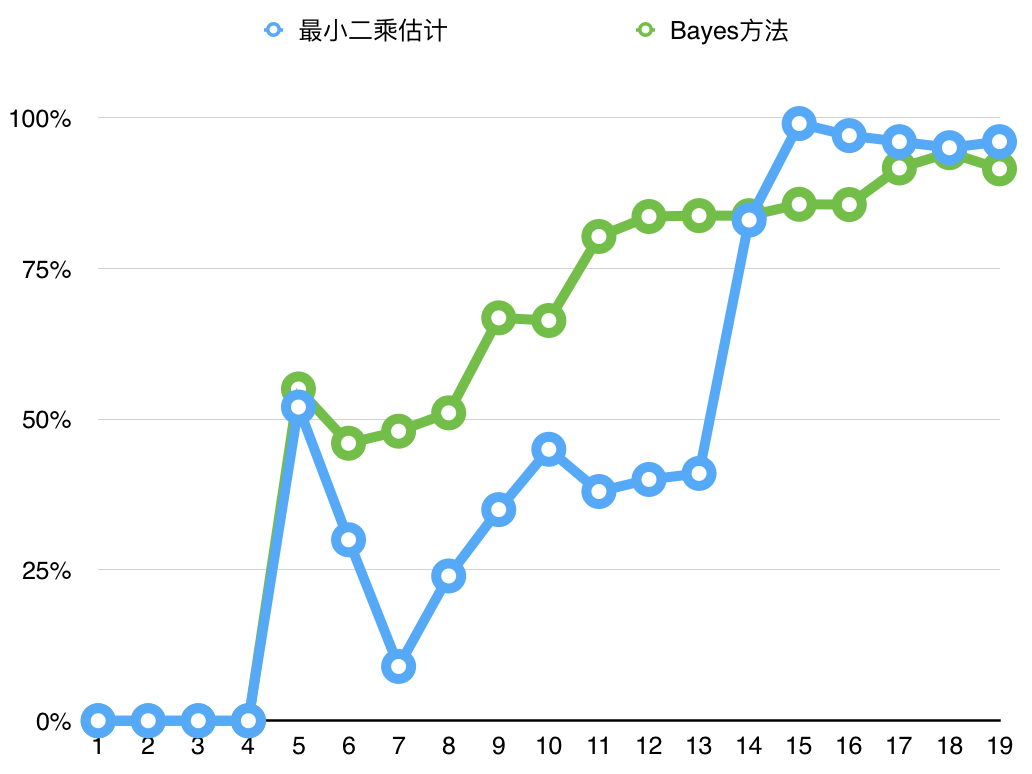
\includegraphics[width=3.5in]{bayes}
  \caption{两种方法对比}
  \label{fig:4.8}
\end{figure}

\subsection{单方向}
利用sumo中的轨迹GPS数据,选取单方向统计5分钟内的轨迹作为输入,之后将估计的两段路的路况与计算出的实际路况进行比对计算出准确率,直行方向和右转方向准确度与轨迹条数的关系见图\ref{fig:4.3}和图\ref{fig:4.4}。

\begin{figure}[H] 
  \centering
  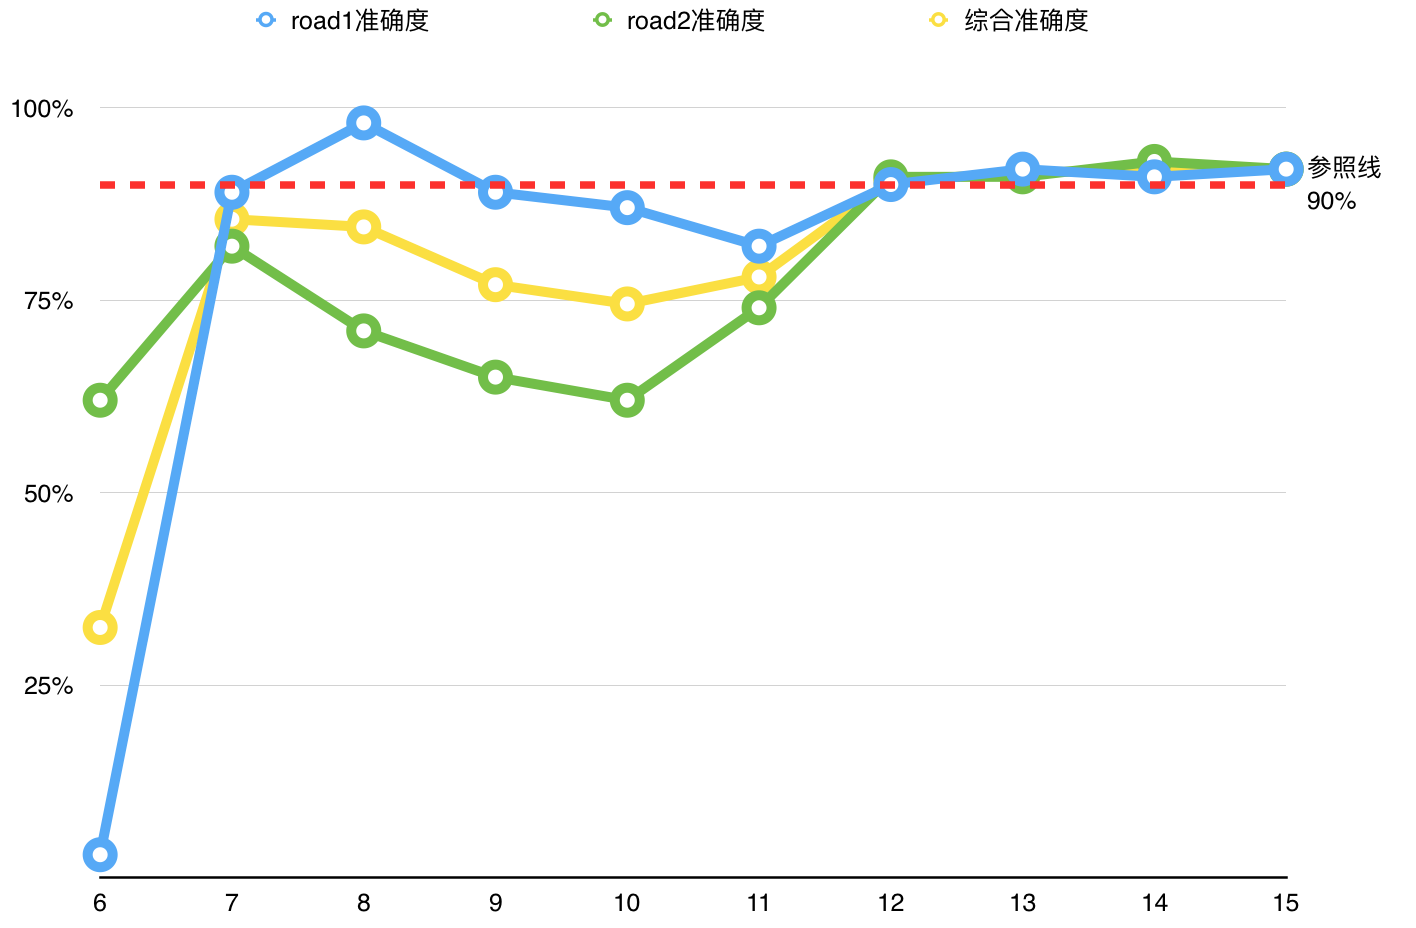
\includegraphics[width=3.5in]{result1}
  \caption{直行方向准确度}
  \label{fig:4.3}
\end{figure}

\begin{figure}[H] 
  \centering
  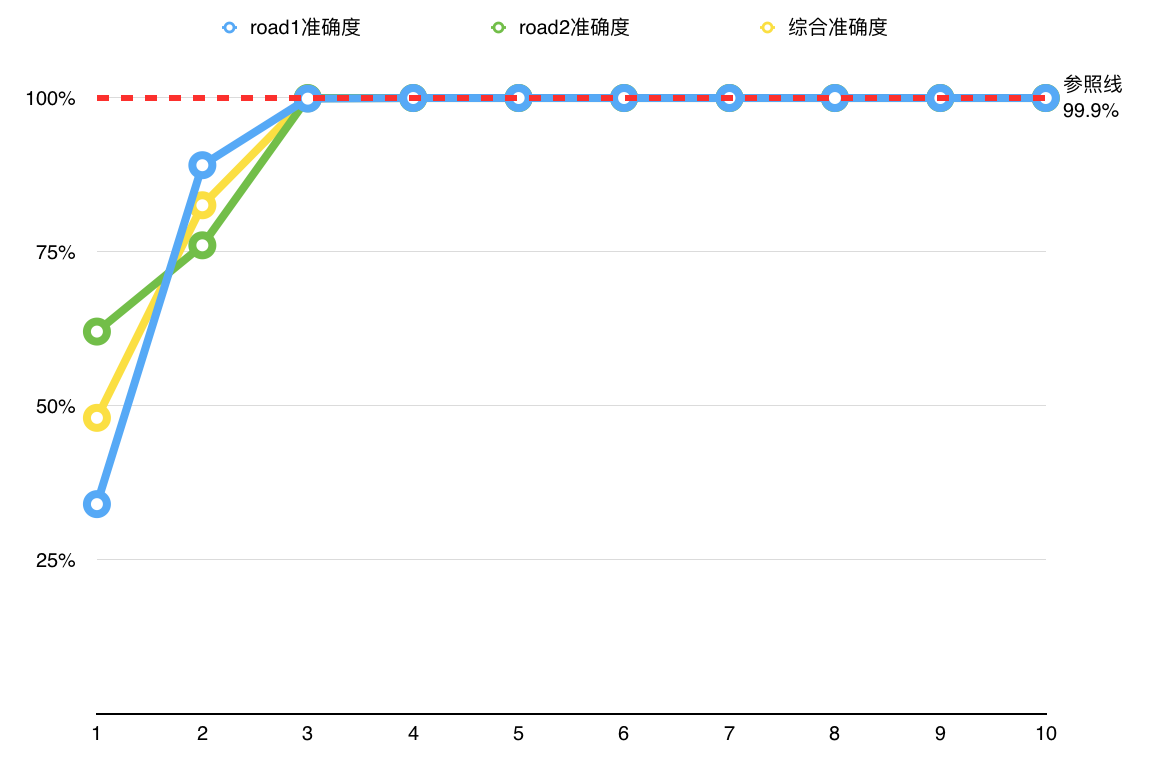
\includegraphics[width=3.5in]{result_right_turn}
  \caption{右转方向准确度}
  \label{fig:4.4}
\end{figure}

从图中我们可以看到直行方向大概需要12条轨迹数据来达到总体90\%的准确率,7条轨迹到11条轨迹之间的结果存在波动,分析数据得出出现波动的原因是其中中间几组数据的信号灯等待时间较长,导致算法回归时直线出现了便宜,数据量再增加直到12条之后,个别数据的偏移不会对总体数据造成很大的影响,左转方向与直行方向的情况基本相同。而右转方向因为无需等待交通信号灯,所以转向延迟比较稳定,采用我们的算法,只需要3条轨迹信息就可以到达99.9\%的正确率。

\subsection{与原有的平滑算法的对比}
当单方向两段路路况存在较大差异时,即一段路堵塞而另一段正常行驶,给出方向有15组GPS轨迹信息,分别使用平滑和线性回归两种算法计算两段路的路况,得出结果如图\ref{fig:4.7}
\begin{figure}[H] 
  \centering
  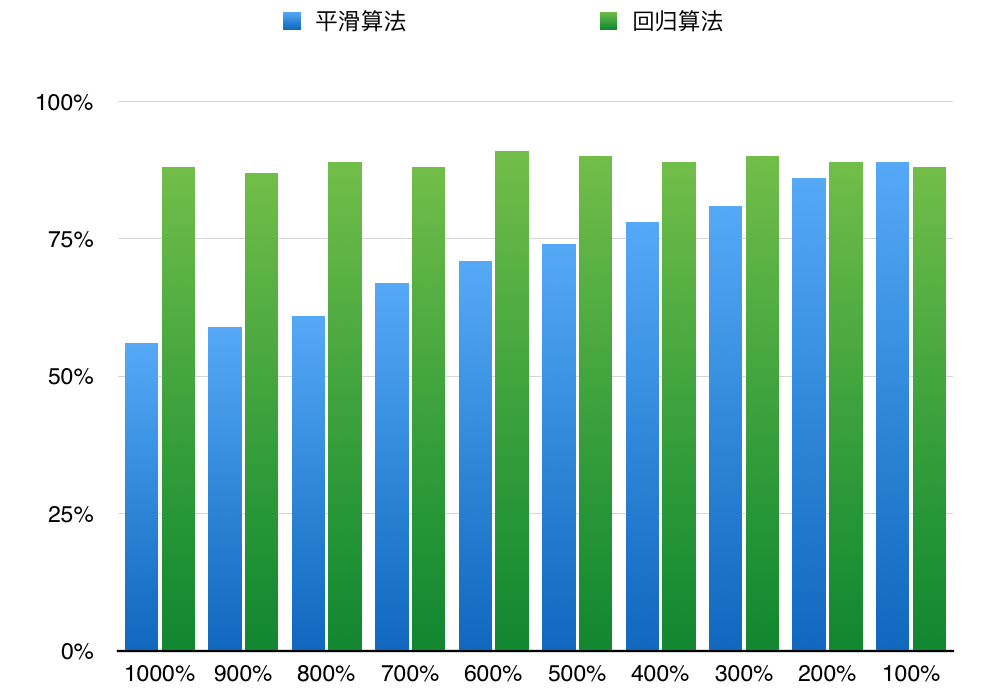
\includegraphics[width=3in]{difference}
  \caption{路况差异较大时两种算法的对比}
  \label{fig:4.7}
\end{figure}
图\ref{fig:4.7}中横坐标为一条轨迹经过两段路段平均速度的比例,纵坐标为路况计算的准确率。实验中我们通过限制一段路的最高速度使得两个路段的畅通程度产生差异。例如横坐标1000\%的点,我们取一段路最高限速为25km\textbackslash h,另一段路最高限速为2.5km\textbackslash h,给出15组车辆轨迹数据,分别用两种方法算出两段路的路况与实际值做对比。我们可以看出,当两个方向的平均速度相差1000\%时,回归算法对比平滑算法优势明显,随着两段路速度差异的变小,算法的准确率差距也逐渐缩小,最后两段路况基本相同时,两种算法的准确率都稳定到90\%左右。

\subsection{三方向混合}
对于经过同一路段的三个方向轨迹信息进行混合,先拿出右转方向的轨迹信息计算出该路段的路况,再将其应用到直行和左转方向的路况计算中,计算下一路段的路况,得出结果如图\ref{fig:4.5}。

\begin{figure}[H] 
  \centering
  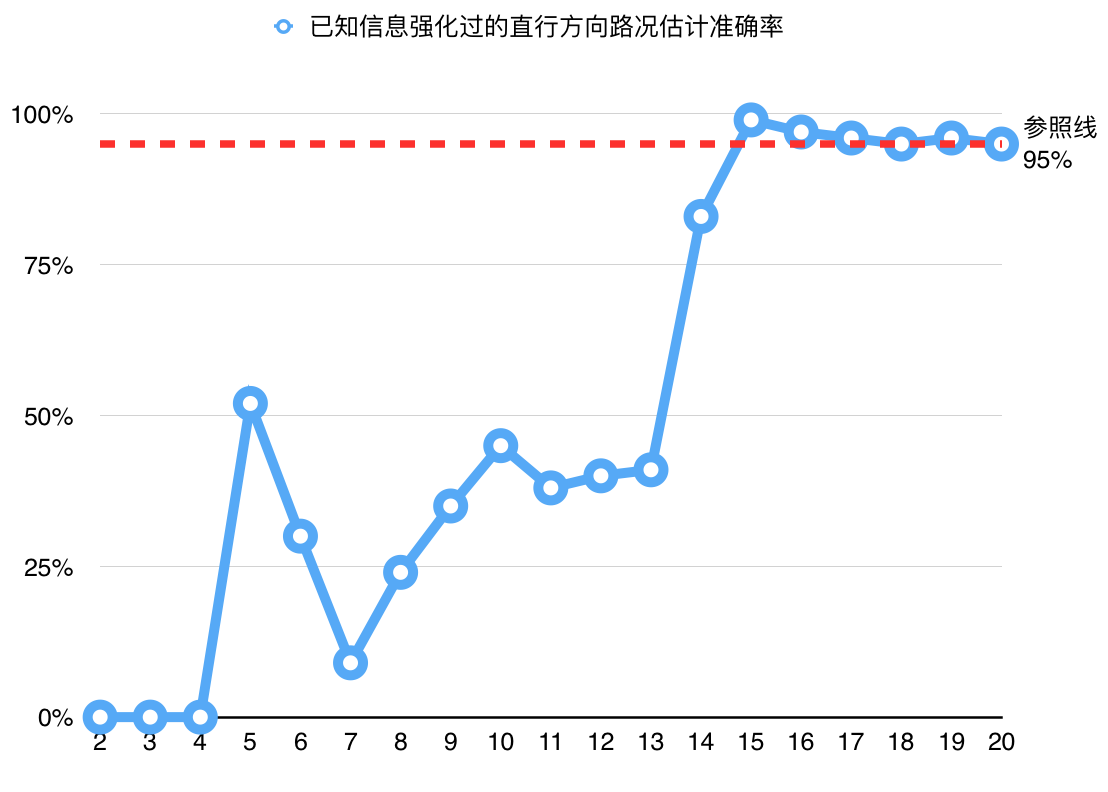
\includegraphics[width=3.5in]{result2}
  \caption{三方向混合准确度}
  \label{fig:4.5}
\end{figure}

从图中我们可以发现,直行方向此时需要15条轨迹数据来达到稳定的准确率,比之前直接对该方向轨迹进行回归的12条还多出三条,这种情况出现的原因是确定前一段路况之后,线性回归又三维降低为二维,但是常数项也就是路口延迟的波动对于我回归的影响会变得更严重,但是达到稳定状态后,我们可以得到比前面更优的结果,准确率为95\%以上,所以我们决定综合使用这两种方法,在轨迹数为14条及以下时直接计算该方向路况,在15条及以上时使用右转方向的既得信息对回归降低维度,得到更精准的结果。

\subsection{全方向混合}
考虑到相对方向的路口信号灯等待和通行周期相同,如果我们得到一个方向的转向延迟,我们就可以把转向延迟应用到其对应方向的计算中,使准确率得到提高。结果如图\ref{fig:4.6}。

\begin{figure}[H] 
  \centering
  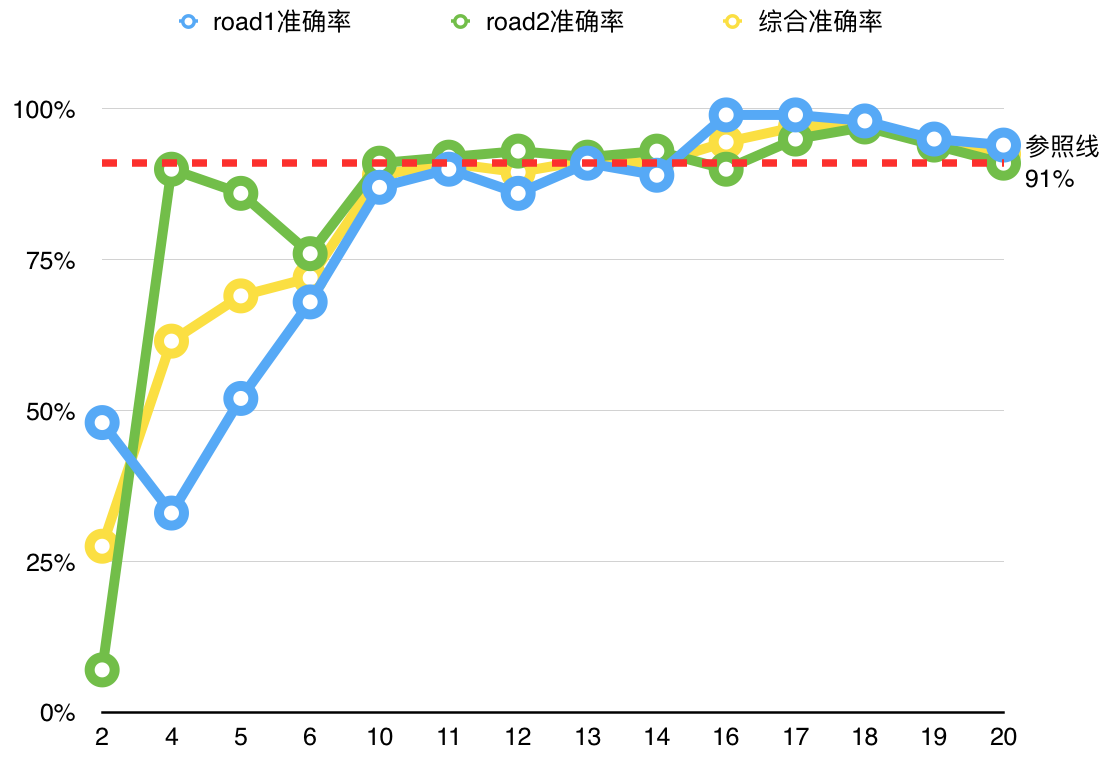
\includegraphics[width=3.5in]{result3}
  \caption{全方向混合准确度}
  \label{fig:4.6}
\end{figure}

从图中我们可以看出得到对应方向的转向延迟信息后,该方向只需要10条轨迹就可以计算出准确率为91\%左右的路况信息,对应方向提供的转向延迟信息可以帮助筛选该方向的数据,规避掉路口信号灯等待时间过长的轨迹信息带来的影响,所以可以使得路况计算所需的轨迹数量减少。

\section{小结}
通过仿真数据的验证,说明了我们的模型对于轨迹数量较多的稀疏数据能够有很高的路况估计准确率。在我们的模型中,对于一个十字路口,最理想的情况是有四个右转方向各三组以上的轨迹数据,这样就能精确地得到8个方向的路况,共需12组轨迹,得到99\%准确率的路况信息。最不理想的情况是没有右转方向的轨迹,这种情况下,我们结合路口对应方向的路况信息,每组对应方向至少需要12+10=22组轨迹信息来得到准确率高于90\%的路况信息,这样加起来就需要至少22*2=44组轨迹信息来得到8个方向的路况。
\chapter{结论}
\label{chap5}

相对于传统的平滑算法,我们的算法改善了相邻两段路况相差较大的情况下的路况计算。使用仿真数据检验了算法的可行性,在轨迹数据较为稀疏,数据量较大的情况下能有很好的结果。当数据量不足的时候对于右转方向也可以有很好的判断。

算法的不足是直行和左转方向的路况判断依赖轨迹的条数比较多,出现这种状况的原因是交通信号灯的随机性比较大,又占到了轨迹总时间的很大比例,造成了数据波动,需要一定的数据量才能拟合回准确值。

未来改进的方向有以下几个方面:
\begin{itemize}
\item 对算法再做优化,降低路口交通信号灯的影响,使得需求的轨迹数量减少。
\item 对算法做扩展,扩充到多个路口的情况,这时需要考虑几个交通信号灯综合作用的情况。
\item 将道路车辆数量,浮动车占到总数量的比例,道路等级,历史路况等信息综合起来考虑,并加入到算法中。
\end{itemize}





%%% 其它部分
\backmatter

%% 本科生要这几个索引,研究生不要。选择性留下。
% 插图索引
\listoffigures
% 表格索引
\listoftables
% 公式索引
\listofequations


%% 参考文献
% 注意:至少需要引用一篇参考文献,否则下面两行可能引起编译错误。
% 如果不需要参考文献,请将下面两行删除或注释掉。
\bibliographystyle{thuthesis}
\bibliography{ref/refs}


%% 致谢
% 如果使用声明扫描页,将可选参数指定为扫描后的 PDF 文件名,例如:
% \begin{acknowledgement}[scan-statement.pdf]
\begin{acknowledgement}
  衷心感谢导师向勇副教授对本人的精心指导。他们的言传身教将使我终生受益。

  感谢清华大学计算机协同工作实验室全体老师和成员的热情帮助和支持。	
  
  感谢 \thuthesis,它的存在让我的论文撰写轻松自在了许多,让我的论文格式规整漂亮了
  许多。
\end{acknowledgement}


%% 附录
\begin{appendix}
%\chapter{外文资料原文}
\label{cha:engorg}

\title{The title of the English paper}

\textbf{Abstract:} As one of the most widely used techniques in operations
research, \emph{ mathematical programming} is defined as a means of maximizing a
quantity known as \emph{bjective function}, subject to a set of constraints
represented by equations and inequalities. Some known subtopics of mathematical
programming are linear programming, nonlinear programming, multiobjective
programming, goal programming, dynamic programming, and multilevel
programming$^{[1]}$.

It is impossible to cover in a single chapter every concept of mathematical
programming. This chapter introduces only the basic concepts and techniques of
mathematical programming such that readers gain an understanding of them
throughout the book$^{[2,3]}$.


\section{Single-Objective Programming}
The general form of single-objective programming (SOP) is written
as follows,
\begin{equation}\tag*{(123)} % 如果附录中的公式不想让它出现在公式索引中,那就请
                             % 用 \tag*{xxxx}
\left\{\begin{array}{l}
\max \,\,f(x)\\[0.1 cm]
\mbox{subject to:} \\ [0.1 cm]
\qquad g_j(x)\le 0,\quad j=1,2,\cdots,p
\end{array}\right.
\end{equation}
which maximizes a real-valued function $f$ of
$x=(x_1,x_2,\cdots,x_n)$ subject to a set of constraints.

\newtheorem{mpdef}{Definition}[chapter]
\begin{mpdef}
In SOP, we call $x$ a decision vector, and
$x_1,x_2,\cdots,x_n$ decision variables. The function
$f$ is called the objective function. The set
\begin{equation}\tag*{(456)} % 这里同理,其它不再一一指定。
S=\left\{x\in\Re^n\bigm|g_j(x)\le 0,\,j=1,2,\cdots,p\right\}
\end{equation}
is called the feasible set. An element $x$ in $S$ is called a
feasible solution.
\end{mpdef}

\newtheorem{mpdefop}[mpdef]{Definition}
\begin{mpdefop}
A feasible solution $x^*$ is called the optimal
solution of SOP if and only if
\begin{equation}
f(x^*)\ge f(x)
\end{equation}
for any feasible solution $x$.
\end{mpdefop}

One of the outstanding contributions to mathematical programming was known as
the Kuhn-Tucker conditions\ref{eq:ktc}. In order to introduce them, let us give
some definitions. An inequality constraint $g_j(x)\le 0$ is said to be active at
a point $x^*$ if $g_j(x^*)=0$. A point $x^*$ satisfying $g_j(x^*)\le 0$ is said
to be regular if the gradient vectors $\nabla g_j(x)$ of all active constraints
are linearly independent.

Let $x^*$ be a regular point of the constraints of SOP and assume that all the
functions $f(x)$ and $g_j(x),j=1,2,\cdots,p$ are differentiable. If $x^*$ is a
local optimal solution, then there exist Lagrange multipliers
$\lambda_j,j=1,2,\cdots,p$ such that the following Kuhn-Tucker conditions hold,
\begin{equation}
\label{eq:ktc}
\left\{\begin{array}{l}
    \nabla f(x^*)-\sum\limits_{j=1}^p\lambda_j\nabla g_j(x^*)=0\\[0.3cm]
    \lambda_jg_j(x^*)=0,\quad j=1,2,\cdots,p\\[0.2cm]
    \lambda_j\ge 0,\quad j=1,2,\cdots,p.
\end{array}\right.
\end{equation}
If all the functions $f(x)$ and $g_j(x),j=1,2,\cdots,p$ are convex and
differentiable, and the point $x^*$ satisfies the Kuhn-Tucker conditions
(\ref{eq:ktc}), then it has been proved that the point $x^*$ is a global optimal
solution of SOP.

\subsection{Linear Programming}
\label{sec:lp}

If the functions $f(x),g_j(x),j=1,2,\cdots,p$ are all linear, then SOP is called
a {\em linear programming}.

The feasible set of linear is always convex. A point $x$ is called an extreme
point of convex set $S$ if $x\in S$ and $x$ cannot be expressed as a convex
combination of two points in $S$. It has been shown that the optimal solution to
linear programming corresponds to an extreme point of its feasible set provided
that the feasible set $S$ is bounded. This fact is the basis of the {\em simplex
  algorithm} which was developed by Dantzig as a very efficient method for
solving linear programming.
\begin{table}[ht]
\centering
  \centering
  \caption*{Table~1\hskip1em This is an example for manually numbered table, which
    would not appear in the list of tables}
  \label{tab:badtabular2}
  \begin{tabular}[c]{|m{1.5cm}|c|c|c|c|c|c|}\hline
    \multicolumn{2}{|c|}{Network Topology} & \# of nodes &
    \multicolumn{3}{c|}{\# of clients} & Server \\\hline
    GT-ITM & Waxman Transit-Stub & 600 &
    \multirow{2}{2em}{2\%}&
    \multirow{2}{2em}{10\%}&
    \multirow{2}{2em}{50\%}&
    \multirow{2}{1.2in}{Max. Connectivity}\\\cline{1-3}
    \multicolumn{2}{|c|}{Inet-2.1} & 6000 & & & &\\\hline
    \multirow{2}{1.5cm}{Xue} & Rui  & Ni &\multicolumn{4}{c|}{\multirow{2}*{\thuthesis}}\\\cline{2-3}
    & \multicolumn{2}{c|}{ABCDEF} &\multicolumn{4}{c|}{} \\\hline
\end{tabular}
\end{table}

Roughly speaking, the simplex algorithm examines only the extreme points of the
feasible set, rather than all feasible points. At first, the simplex algorithm
selects an extreme point as the initial point. The successive extreme point is
selected so as to improve the objective function value. The procedure is
repeated until no improvement in objective function value can be made. The last
extreme point is the optimal solution.

\subsection{Nonlinear Programming}

If at least one of the functions $f(x),g_j(x),j=1,2,\cdots,p$ is nonlinear, then
SOP is called a {\em nonlinear programming}.

A large number of classical optimization methods have been developed to treat
special-structural nonlinear programming based on the mathematical theory
concerned with analyzing the structure of problems.
\begin{figure}[h]
  \centering
  
\includegraphics{thu-lib-logo}
  \caption*{Figure~1\quad This is an example for manually numbered figure,
    which would not appear in the list of figures}
  \label{tab:badfigure2}
\end{figure}

Now we consider a nonlinear programming which is confronted solely with
maximizing a real-valued function with domain $\Re^n$.  Whether derivatives are
available or not, the usual strategy is first to select a point in $\Re^n$ which
is thought to be the most likely place where the maximum exists. If there is no
information available on which to base such a selection, a point is chosen at
random. From this first point an attempt is made to construct a sequence of
points, each of which yields an improved objective function value over its
predecessor. The next point to be added to the sequence is chosen by analyzing
the behavior of the function at the previous points. This construction continues
until some termination criterion is met. Methods based upon this strategy are
called {\em ascent methods}, which can be classified as {\em direct methods},
{\em gradient methods}, and {\em Hessian methods} according to the information
about the behavior of objective function $f$. Direct methods require only that
the function can be evaluated at each point. Gradient methods require the
evaluation of first derivatives of $f$. Hessian methods require the evaluation
of second derivatives. In fact, there is no superior method for all
problems. The efficiency of a method is very much dependent upon the objective
function.

\subsection{Integer Programming}

{\em Integer programming} is a special mathematical programming in which all of
the variables are assumed to be only integer values. When there are not only
integer variables but also conventional continuous variables, we call it {\em
  mixed integer programming}. If all the variables are assumed either 0 or 1,
then the problem is termed a {\em zero-one programming}. Although integer
programming can be solved by an {\em exhaustive enumeration} theoretically, it
is impractical to solve realistically sized integer programming problems. The
most successful algorithm so far found to solve integer programming is called
the {\em branch-and-bound enumeration} developed by Balas (1965) and Dakin
(1965). The other technique to integer programming is the {\em cutting plane
  method} developed by Gomory (1959).

\hfill\textit{Uncertain Programming\/}\quad(\textsl{BaoDing Liu, 2006.2})

\section*{References}
\noindent{\itshape NOTE: These references are only for demonstration. They are
  not real citations in the original text.}

\begin{translationbib}
\item Donald E. Knuth. The \TeX book. Addison-Wesley, 1984. ISBN: 0-201-13448-9
\item Paul W. Abrahams, Karl Berry and Kathryn A. Hargreaves. \TeX\ for the
  Impatient. Addison-Wesley, 1990. ISBN: 0-201-51375-7
\item David Salomon. The advanced \TeX book.  New York : Springer, 1995. ISBN:0-387-94556-3
\end{translationbib}

\chapter{外文资料的调研阅读报告或书面翻译}

\title{英文资料的中文标题}

{\heiti 摘要:} 本章为外文资料翻译内容。如果有摘要可以直接写上来,这部分好像没有
明确的规定。

\section{单目标规划}
北冥有鱼,其名为鲲。鲲之大,不知其几千里也。化而为鸟,其名为鹏。鹏之背,不知其几
千里也。怒而飞,其翼若垂天之云。是鸟也,海运则将徙于南冥。南冥者,天池也。
\begin{equation}\tag*{(123)}
 p(y|\mathbf{x}) = \frac{p(\mathbf{x},y)}{p(\mathbf{x})}=
\frac{p(\mathbf{x}|y)p(y)}{p(\mathbf{x})}
\end{equation}

吾生也有涯,而知也无涯。以有涯随无涯,殆已!已而为知者,殆而已矣!为善无近名,为
恶无近刑,缘督以为经,可以保身,可以全生,可以养亲,可以尽年。

\subsection{线性规划}
庖丁为文惠君解牛,手之所触,肩之所倚,足之所履,膝之所倚,砉然响然,奏刀騞然,莫
不中音,合于桑林之舞,乃中经首之会。
\begin{table}[ht]
\centering
  \centering
  \caption*{表~1\hskip1em 这是手动编号但不出现在索引中的一个表格例子}
  \label{tab:badtabular3}
  \begin{tabular}[c]{|m{1.5cm}|c|c|c|c|c|c|}\hline
    \multicolumn{2}{|c|}{Network Topology} & \# of nodes &
    \multicolumn{3}{c|}{\# of clients} & Server \\\hline
    GT-ITM & Waxman Transit-Stub & 600 &
    \multirow{2}{2em}{2\%}&
    \multirow{2}{2em}{10\%}&
    \multirow{2}{2em}{50\%}&
    \multirow{2}{1.2in}{Max. Connectivity}\\\cline{1-3}
    \multicolumn{2}{|c|}{Inet-2.1} & 6000 & & & &\\\hline
    \multirow{2}{1.5cm}{Xue} & Rui  & Ni &\multicolumn{4}{c|}{\multirow{2}*{\thuthesis}}\\\cline{2-3}
    & \multicolumn{2}{c|}{ABCDEF} &\multicolumn{4}{c|}{} \\\hline
\end{tabular}
\end{table}

文惠君曰:“嘻,善哉!技盖至此乎?”庖丁释刀对曰:“臣之所好者道也,进乎技矣。始臣之
解牛之时,所见无非全牛者;三年之后,未尝见全牛也;方今之时,臣以神遇而不以目视,
官知止而神欲行。依乎天理,批大郤,导大窾,因其固然。技经肯綮之未尝,而况大坬乎!
良庖岁更刀,割也;族庖月更刀,折也;今臣之刀十九年矣,所解数千牛矣,而刀刃若新发
于硎。彼节者有间而刀刃者无厚,以无厚入有间,恢恢乎其于游刃必有余地矣。是以十九年
而刀刃若新发于硎。虽然,每至于族,吾见其难为,怵然为戒,视为止,行为迟,动刀甚微,
謋然已解,如土委地。提刀而立,为之而四顾,为之踌躇满志,善刀而藏之。”

文惠君曰:“善哉!吾闻庖丁之言,得养生焉。”


\subsection{非线性规划}
孔子与柳下季为友,柳下季之弟名曰盗跖。盗跖从卒九千人,横行天下,侵暴诸侯。穴室枢
户,驱人牛马,取人妇女。贪得忘亲,不顾父母兄弟,不祭先祖。所过之邑,大国守城,小
国入保,万民苦之。孔子谓柳下季曰:“夫为人父者,必能诏其子;为人兄者,必能教其弟。
若父不能诏其子,兄不能教其弟,则无贵父子兄弟之亲矣。今先生,世之才士也,弟为盗
跖,为天下害,而弗能教也,丘窃为先生羞之。丘请为先生往说之。”
\begin{figure}[h]
  \centering
  
\includegraphics{thu-whole-logo}
  \caption*{图~1\hskip1em 这是手动编号但不出现索引中的图片的例子}
  \label{tab:badfigure3}
\end{figure}

柳下季曰:“先生言为人父者必能诏其子,为人兄者必能教其弟,若子不听父之诏,弟不受
兄之教,虽今先生之辩,将奈之何哉?且跖之为人也,心如涌泉,意如飘风,强足以距敌,
辩足以饰非。顺其心则喜,逆其心则怒,易辱人以言。先生必无往。”

孔子不听,颜回为驭,子贡为右,往见盗跖。

\subsection{整数规划}
盗跖乃方休卒徒大山之阳,脍人肝而餔之。孔子下车而前,见谒者曰:“鲁人孔丘,闻将军
高义,敬再拜谒者。”谒者入通。盗跖闻之大怒,目如明星,发上指冠,曰:“此夫鲁国之
巧伪人孔丘非邪?为我告之:尔作言造语,妄称文、武,冠枝木之冠,带死牛之胁,多辞缪
说,不耕而食,不织而衣,摇唇鼓舌,擅生是非,以迷天下之主,使天下学士不反其本,妄
作孝弟,而侥幸于封侯富贵者也。子之罪大极重,疾走归!不然,我将以子肝益昼餔之膳。”


\chapter{其它附录}
前面两个附录主要是给本科生做例子。其它附录的内容可以放到这里,当然如果你愿意,可
以把这部分也放到独立的文件中,然后将其 \cs{input} 到主文件中。

\chapter{外文资料书面翻译}

\title{应用于实时交通传感应用基于隐马尔科夫模型的在线地图匹配}


\textbf{摘要:} 在许多智能交通系统(ITS)应用程序中,探测车辆的数据来源,一个关键的步骤是准确地将GPS轨迹实时地映射到道路网络。这个过程被称为地图匹配,通常需要考虑数据的噪声和稀疏性,因为(1)高度精确的GPS轨迹信息非常稀有,以及(2)密集轨迹对于实况传输和存储是昂贵的。

我们提出了一种基于对噪声和稀疏性鲁棒的隐马尔可夫模型(HMM)的在线地图匹配算法。我们集中在现有的基于HMM的算法的两个改进:(1)使用最佳局部化策略,可变滑动窗口(VSW)方法,保证在不确定的未来输入下的在线解决方案质量,和(2)使用机器学习的空间,时间和拓扑信息。我们使用在城市和农村地区的公交路线上收集的现场测试数据来评估我们的算法的准确性。此外,我们还研究了在处理实时输入流时精度和输出延迟之间的关系。

在我们对现场测试数据的测试中,VSW在精度和输出延迟方面都优于传统的定位方法。我们的研究结果表明,它可以应用于对延迟要求较为苛刻的应用程序,如交通流量传感。

\section{引言}
由大量车辆收集的实时传感器数据,例如城市地区的出租车和公共汽车,为交通感测,交通事故检测,旅行时间预测[3],车辆管理[4]和路线建议[5],[6]。这些系统的可用性取决于通过可用的地图匹配算法提取的数据的可靠性,地图匹配算法做的就是将GPS轨迹投影到数字地图上的相应路段。

诸如时间戳,位置和速度的信息通常由探测车辆记录。 然而,处理这些大量数据所需的高额到难以负担的存储和带宽导致了现在收集稀疏样本的做法,间隔范围从几十秒到几分钟[7]。此外,已知安装在这些探头上的传感器容易出现各种错误[7],例如不精确的位置和速度测量,重复传输和时间戳不匹配。在诸如交通感测的实时应用中,还要求在未来数据点未给出的时候就执行地上的地图匹配,即算法必须在线。可靠的在线地图匹配算法因此必须考虑这些问题并且保证精度和及时性高的输出。

地图匹配算法被定性为全局或增量/在线。全局算法在生成解之前对整个输入轨迹进行批处理。增量/在线算法采用将输入轨迹划分为更小段并按顺序处理的局部化策略,有时导致次优解。在地图匹配中应用的技术包括几何分析[12],信念函数理论[13],扩展卡尔曼滤波器[14]和隐马尔可夫模型[11] [15] [16]。这些方法的优势和局限性已在[9]中综述。特别地,已经采用基于HMM的算法及其变体[10],[17]用于同时评估实际映射的多个假设的能力,以便找到最终的最大似然解。这些方法已经被证明可以抵抗高度噪声测量,例如来自GSM塔的位置指纹[16],并且它们的精度随着轨迹的时间稀疏度的增加而退化[10],[15],[17]。

我们提出的在线HMM(OHMM)地图匹配算法受到最近基于HMM的方法[10],[15] - [17]的启发。我们解决了在以前的相关工作中没有集中的两个具体问题:(i)需要一个在线算法来管理精度和输出延迟之间的权衡,以及(ii)多个评分函数的融合以估计转换可能性。

大多数现有的增量/在线算法使用简单的定位策略,例如固定滑动窗口和固定深度递归预测。滑动窗口方法简单地将轨迹划分为固定大小的输入序列并且独立地处理它们。较大的窗口尺寸导致更好的精度[10],[17]但更长的输出延迟,反之亦然。递归预测方法将每个点的决定延迟固定数量的步长,以评估未来路径替代方案[18]。这两种方法虽然易于实现,但可能导致次优解决方案和长输出延迟。当地图匹配算法在实时输入流上操作并且需要在短时间窗口内产生输出时,这显然是不可行的。受实时应用需求的驱使,我们提出了一个最优的局部化策略,使用可变滑动窗口(VSW)将输入分成更小的子问题,并证明找到全局最优解。我们的方法在概念上类似于在线维特比算法[19],[20]。此外,我们还开发了VSW的次优变体,其提供对延迟性能的最坏情况保证。在第五节中,我们将使用定长滑动窗口(FSW)方法作为基准来比较这两种方法的性能。

其次,我们推导了一种概率评分机制,其在HMM中的表现和转移概率的建模中结合了各种传感器数据和拓扑信息:(i)GPS坐标(ii)车辆速度(iii)速度限制(iv)推断的车辆前进方向,以及(vi)拓扑约束。我们使用支持向量机(SVM)来学习转移概率函数,而不是选择简单的先验模型[10],[15],[17],然后估计其参数。这种方法的主要优点是它提供了一个数据驱动的框架,用于集成多个过渡评分函数。

我们使用在新加坡包括农村和城市地区的4条公交线路上收集的现场测试数据来评估我们的方法的性能。性能是根据精度和输出延迟标准来测量的。我们的研究结果表明,当操作在实时输入流时,所提出的算法实现了优化或接近最优解,实际上具有低输出延迟。

本文结构如下。第二节根据HMM来制定地图匹配问题。方法将在第三节中描述。我们的实验设置在第四部分解释。结果在第五节中介绍。最后,第六部分总结了我们的贡献,并讨论了未来工作的空间。


\section{地图匹配问题}

\subsection{问题定义}

\textbf{定义1}:轨迹,$T=(t_{n} | n=1,...,N)$,是由车辆收集的N个数据点组成的序列。每个轨迹点由其经度$(t_{n}.lon)$,纬度$(t_{n}.lat)$,速度$(t_{n}.v)$和时间戳$(t_{n}.t)$指定。

\textbf{定义2}:段落,$r=(p_{m} | m=1,..,M)$,是一条M点折线表示的道路段曲线。它由连接顶点的一系列线段$p_{1},…,p_{m}$组成。按顺序,其中每个顶点由其经度和纬度指定。 段落也由其道路宽度(r.w),速度限制(r.v)和双向行驶(r.d)的允许性定义(r.d=\{true,flase\})。

\textbf{定义3}:数字地图,$G=\{r_{k} | k=1,..,K\}$,是一组代表K个段落的集合。

给定轨迹T,地图匹配的目标是找到T每个轨迹点到G中段落的对应关系。

\subsection{HMM方法}
在基于HMM的地图匹配算法中,候选路径被顺序地生成并基于它们的似然性来评估。当遇到新的轨迹点时,解决方案的过去的假设被扩展以考虑新的观测值。在最后阶段的所有候选中,具有最高联合概率的幸存路径然后被选择为最终解。

对于每个轨迹点,我们首先从该数据最有可能被采集的地点识别一组候选道路段落。这些候选中的每一个表示为马尔可夫链中的隐藏状态,并且具有表现概率,其是在候选段是真实匹配的情况下观察GPS点的可能性。直观地,如果点被发现更接近它,​​我们将给段更高的概率。然后,我们计算链中每对相邻隐藏状态的转移概率,使得后者的概率仅取决于前者,因此服从马尔可夫假设。我们的目标是找到具有最高联合表现和传输概率的马尔科夫链上的最大似然路径。该过程如图1所示。

正式地,我们将表现概率表示为p(t | h),其是给定隐藏状态(段)的观察到轨迹点t的概率。 从隐藏状态到隐藏状态的转移概率是f(s,h)。给定一个N个点轨迹,隐藏状态的似然序列,$T=(t_{n} | n=1,…,N)$,隐藏状态的似然序列,$S^{*}=(S_{n}\in A_{n} |n=1,...,N)$满足以下递推关系。

\begin{equation*}
V_{n,h}=p(t_{n}h)\max_{s\in A_{n-1}} \{f(s,h)V_{n-1,s}\}.
\end{equation*}

这里$V_{0,h}=p(t_{0}|h)$和$A_{n}$表示第n阶段的隐藏状态集合 。然后,我们可以从最后一个元素中找到$S^{*}$,$s_{N}=\arg\max_{h\in A_{n}}\{V_{N,h}\}$,向后工作找到最大联合概率序列$S_{N-1}$,...$S_{1}$。 我们在第3-E节将提供一个在线算法找到$S^{*}$。


\section{OHMM地图匹配算法}

\subsection{算法的基本流程}
\begin{itemize}
\item 对于每个轨迹点,找到围绕其半径为50m的所有候选分段。 施加该阈值的原因是双重的:(1)丢弃具有非常低的表现概率(低于$10^{-4}$的范围)的所有候选,以及(2)避免由于过多候选而导致执行速度的惩罚。

\item 针对每个候选分段(隐藏状态)计算表现概率,而将转移概率分配给在隐藏状态上发生的每个边缘。

\item VSW算法在更新的Markov链上执行回溯,并给出部分求解(如果可用)。 否则,输出将延迟一个阶段。

\item 对下一个轨迹点重复上述过程。 当到达最后一点时,算法终止。
\end{itemize}

\subsection{表现概率}
对于在轨迹点附近找到的每个候选分段,我们用1D高斯函数对其观测概率进行建模,如下所示。

\begin{equation*}
p(observation)=\frac{1}{2w}{\int_{-w}^{w}}\frac{1}{\sqrt{2\pi\sigma_{g}^{2}}}e^{-\frac{(l-d)^{2}}{2\pi\sigma_{g}^{2}}}dl.
\end{equation*}

这里w是指道路r的半宽(w=0.5*r.w),d是指t和r间点到曲线之间的大圆距离,$\sigma_{g}$是GPS误差的估计标准偏差。 虽然GPS误差已知具有非高斯分布,我们采用这种模型是因为它易于实现和在之前的工作被证明有效[10],[15],[17]。 我们的方法是不同的,因为我们也考虑道路宽度。 这将允许我们更好地在路段之间区分,特别是在路口。

此外,基于假设驾驶员不大可能大大超过速度限制,我们引入超速的惩罚机制。 目的是帮助区分从相同交叉点分支出的可能具有不同速度限制的紧密间隔的平行道路。 我们注意到在这些情况下,单独的位置测量不足以区分段落,因为记录的轨迹点可能落在它们之间。 我们定义惩罚函数S如下,

\begin{equation*}
S(v_{t},v_{r})=\frac{v_{r}}{max(0,v_{t}-v_{r})+v_{r}}.
\end{equation*}

这里vt指传感器记录的时间,而vr指该路段的限制速度。如果遵守了速度限制,则$max(0,v_{t}-v_{r})=0$。(即惩罚机制不启动)。结合(2)和(3),我们定义表现概率,p(t | r)如下

\begin{equation*}
p(t|r)=S(v_{t},v_{r})p(oberservation).
\end{equation*}

\subsection{转移概率}
令i,j分别表示归属于两个连续轨迹点$t_{n}$和$t_{n+1}$的一对候选段,其中$i\in A_{n}$、$j\in A_{n-1}$。 我们将内插路径$P_{i\to j}$定义为当从i行进到j时车辆最可能采取的段的序列。 假设驾驶员选择最短路程的路(路径距离短的被选择可能性高),我们可以使用A*路径寻找算法找到插值路径[21]。 对于K个片段的给定序列,$P_{i\to j}$中的$(r_{1},…,r_{k})$,我们设计如下的两个评分函数,

\textbf{方法1}:距离差异函数T测量传感器推测的行进距离和插值路径长度之间的差异,

\begin{equation*}
T(d_{i\to j},D_{i\to j})=\frac{|d_{i\to j}-D_{t\to j}|}{D_{i\to j}},
\end{equation*}

这里$d_{i\to j}=\overline{v}_{i\to j}\Delta t$是车辆在时间间隔,以平均速度$\overline{v}_{i\to j}$行驶的距离,而$D_{i\to j}$是$P_{i\to j}$的路径长度。上面的方法1通过比较其长度与推测(DR)估计评估了假设路径$P_{i\to j}$的可行性。如果$P_{i\to j}$是真实路径,差异会被假定为接近于零。

\textbf{方法2}:选用动量变化函数M测量车辆对于在$P_{i\to j}$中采取的每个路段所引起的平均动量变化,

\begin{equation*}
M(v_{0},v_{1},l_{1},...,v_{k},l_{k})=\frac{\sum_{i}^{K}l_{i}||v_{i}-v_{i-1}||}{\overline{v}_{i\to j}\sum_{i}^{K}l_{i}},
\end{equation*}

其中$(v_{1},..,v_{k})$是$P_{i\to j}$中每个段的车辆的速度矢量,并且$(l_{1},...,l_{k})$是相应的段长度。我们假设矢量幅度随时间从$|v_{1}|$线性变化到$|v_{n}|$ ,而它们的方向与段曲线平行。注意,附加参数v0是从先前转换的终端速度继承的初始速度矢量。通过类似的逻辑,我们将使用$v_{k}$,当前终端速度作为下一转换中的初始速度,等等。图2示出了该概念。上述措施2可以被描述为“平滑因子”,其对由许多突然转弯组成的不可行转移做惩罚。

上面介绍的评分函数T和M为转变$i\to j$提供两种不同的“适合度度量”。这表明,可以通过将这两个度量融合在一起来导出转移概率。 我们使用标记为正确或不正确转换的实例训练支持向量机(SVM)分类器,其中特征向量由测量1和测量2给出的分量分数组成。利用该分类方法,$P_{i\to j}$是输入得分组合属于“正确转换”类别的概率。 我们将在第4-B节更详细地描述训练过程。

\subsection{在线维特比算法}
我们的目标是使用增量法找到全局地图匹配解决方案。 这意味着该算法需要在不知道未来输入的情况下沿着马尔可夫链进行不可逆的在线决策,同时确保部分解在组合时产生全局最优解。 为了实现这一点,我们应用在线动态规划来解决(1)中的递推关系。 关键的见解是,当当前幸存路径在马尔科夫链中的某点(收敛点)收敛时,所有未来的幸存路径将包含直到收敛点的相同子路径。 相关证据可在[19]和[20]中找到。

我们制定我们的OHMM算法的伪码如下。算法1(OHMM地图匹配)递增地处理轨迹点,并且在每个阶段,它输出算法2返回的部分解,如果可用的话。否则,它给出一个空输出,并引发一个延迟阶段。算法2(在线维特比算法)检查在解链中是否存在任何收敛点,并返回到该点的最大似然子序列(如果有的话)。

方便地描述算法1和2在滑动窗口方面的工作原理。当在由窗口覆盖的马尔科夫链中的任何地方找到收敛点时,窗口随着新的轨迹点被处理并从后面收缩而向前扩展。注意,滑动窗口的大小可以根据状态空间的结构而变化,因此名称可变滑动窗口。图3示出了VSW的工作原理。

然而,VSW的一个缺点是不能保证最坏情况的窗口大小;因此在极端情况下输出延迟可以是任意大的。我们通过设置窗口大小的上限来修改算法1,使得当达到阈值时,算法将输出直到当前阶段的最大似然解。我们将标记这个修改的方法有界滑动窗(BVSW)方法。但是与VSW不同,这种方法可能导致次优解决方案。

\section{实验装置}

\subsection{现场测试数据}
使用支持GPS的智能手机,我们收集了在新加坡的4条预定的公共汽车路线的地面实况数据,如图4所示。由于我们关心地图匹配结果的路径精度(将在第6-C节中定义),因此对实际测试路径(地面实况路径)的了解足以使我们验证算法。为了比较不同环境条件下的表现,我们选择了涵盖新加坡农村和城市地区的4条路线。农村路线(R1和R2)涉及较少的转弯,并且主要包括通过开放区域的直线路线,例如高速公路。城市路线(U1和U2)除了更加高度分支外,还包括密集地包含高层建筑的城市街区。 R1,R2,U1和U2的长度分别为36.3km,11.3km,27.3km和32.5km。此外,为了模拟变化的采样频率的轨迹,我们以10秒到5分钟的采样间隔对我们的原始数据(每1-3秒记录一次)进行二次采样。

\subsection{训练和参数估计}

参数$\sigma_{g}$需要在(2)中估计体现概率,并且转换概率需要SVM训练。

我们通过分析我们的地面实际数据的扰动来估计$\sigma_{g}$。 对于每个轨迹点,我们计算该点离其最近路段中心的大圆距离。 然后,基于距离的中值绝对偏差(MAD)计算标准偏差,

\begin{equation*}
\sigma_{g}=1.4826 median_{i}(|d_{i}-median_{j}(d_{j})|).
\end{equation*}

这里$d_{i}$表示单个轨迹点与其匹配段之间的垂直距离。 距离的分布允许我们估计地面真实路径周围的轨迹点的一维扰动。 注意在(7)中,MAD由常数因子1.4826缩放,因为我们假设GPS测量误差是正态分布的。 我们采用MAD方法因为它对抗能够更好地对抗数据集中的异常值。 在[7],[15]中采用了相同的估计标准差的方法。 基于整个数据集,我们获得$\sigma_{g}$= 6.86m。

为了推断转移概率,我们使用3,000个标记的实例训练SVM分类器,其中每个实例对应于正确的转换(类别标记为'1')或不正确的转换(类别标记为'2')。每个实例是2D特征向量 (5)和(6)计算得到的得分值,并且两个分量被缩放为[0,1]。 缩放函数是$(1+x)^{-1}$,其中x是特征的任一分量。 使用网格搜索参数空间和5重交叉验证,我们发现参数的最佳组合为C = 0.25和g = 0.5,其中C是软边际参数,g是径向基函数(RBF)内核参数。 训练结果如图5所示。

\subsection{性能评价}
我们将使用两个性能度量来评估我们的算法:精度和输出延迟。

精度被定义为地面实际路径中正确匹配的轨迹点的分数。当轨迹点被映射到包含在地面实况路径中的任何道路段时,记录正确的匹配。这种准确性的测量避免了惩罚“边界类”,其中点位于路口的正中间。我们注意到,精确地确定收集每个轨迹点的路段是不切实际的,原因在于两个原因:(i)“边界类”可以归因于交叉点的任一出口上的路段,以及(ii)可能的误校准的数字地图。因此,路径精度测量是更合适的评估标准。

输出延迟是算法对每个轨迹点引起的平均输出延迟。它通过在获得匹配结果之前花费的时间来量化。

测试如下进行:

\begin{itemize}

\item 我们对农村和城市测试路线的不同采样间隔的测试轨迹执行地图匹配,范围从3秒到5分钟。 对于每个路由类别,我们聚合两个测试路由获得的结果。

\item 我们比较了三种定位策略在精度和输出延迟方面:VSW,BVSW和FSW。 对于BVSW和FWS,测试了不同的窗口尺寸。 对于每个窗口大小,我们聚集整组测试数据的结果(4个测试路由,采样间隔在10秒到5分钟之间)。

\end{itemize}

\section{结果}

图6展示了城乡测试路线的地图匹配精度的比较。 结果表明,除了大于4分钟的抽样间隔外,农村路线的准确性比城市路线的准确度大约为5%。 以小于1分钟的间隔,两条路线的精度都高于0.9。 在这两种情况下,精度随着采样间隔的增加而恶化。

图7和图8中,虚线表示使用VSW定位策略实现的最优结果。 BVSW方法在w = 8及以上时收敛到0.921的最佳精度。 在所有情况下,FSW方法给出一致的较低精度,并且没有收敛到最优解,即使在w = 20。

在图8中,VSW的平均输出延迟为82s。与FSW相比,它实现了显着更低的延迟,而没有折衷解决方案的最优性。 使用BVSW,在4和以上的窗口大小的延迟性能中没有显着的优点。 这表明马尔可夫链中的大多数决策点发生在达到窗口界限之前。 在FSW的情况下,延迟与窗口大小成比例地增加,但是在某个阈值点之后精度增益减小到几乎为零。




\section{结论和未来工作}

在本文中,我们描述了一种用于地图匹配的在线算法,并分析其在地面实况数据上的性能。我们设计了VSW和BVSW方法来寻找在线解决方案。两者在精度和输出延迟方面都优于先前基于HMM的算法中使用的传统FSW定位策略。我们还开发了一种数据驱动的方法,用于推断在地图匹配过程中融合传感器测量和拓扑信息的转换概率。总而言之,这些方法提供了用于设计基于在线HMM的地图匹配算法的一般框架,其适合于使用浮动车辆数据的实时应用。算法的其它变体可以在估计体现和转移概率时结合附加的传感器数据,例如加速度和高度测量。

对于未来的工作,我们可以探索地图匹配算法的设计与动态参数检测和适应不同的环境设置,如在城市或农村地区,其中GPS准确性可能会变化。传感器信息,例如用于GPS测量的精度(DOP)值的稀释可能被证明对于实现这个目标是有用的。此外,我们建议更好的方法[22]内插轨迹点,而不是假设它们之间的最短路径。对实际行进路径的更好近似可以提高地图匹配精度。
\end{appendix}

%% 个人简历
%\begin{resume}

  \resumeitem{个人简历}

  xxxx 年 xx 月 xx 日出生于 xx 省 xx 县。

  xxxx 年 9 月考入 xx 大学 xx 系 xx 专业,xxxx 年 7 月本科毕业并获得 xx 学士学位。

  xxxx 年 9 月免试进入 xx 大学 xx 系攻读 xx 学位至今。

  \researchitem{发表的学术论文} % 发表的和录用的合在一起

  % 1. 已经刊载的学术论文(本人是第一作者,或者导师为第一作者本人是第二作者)
  \begin{publications}
    \item Yang Y, Ren T L, Zhang L T, et al. Miniature microphone with silicon-
      based ferroelectric thin films. Integrated Ferroelectrics, 2003,
      52:229-235. (SCI 收录, 检索号:758FZ.)
    \item 杨轶, 张宁欣, 任天令, 等. 硅基铁电微声学器件中薄膜残余应力的研究. 中国机
      械工程, 2005, 16(14):1289-1291. (EI 收录, 检索号:0534931 2907.)
    \item 杨轶, 张宁欣, 任天令, 等. 集成铁电器件中的关键工艺研究. 仪器仪表学报,
      2003, 24(S4):192-193. (EI 源刊.)
  \end{publications}

  % 2. 尚未刊载,但已经接到正式录用函的学术论文(本人为第一作者,或者
  %    导师为第一作者本人是第二作者)。
  \begin{publications}[before=\publicationskip,after=\publicationskip]
    \item Yang Y, Ren T L, Zhu Y P, et al. PMUTs for handwriting recognition. In
      press. (已被 Integrated Ferroelectrics 录用. SCI 源刊.)
  \end{publications}

  % 3. 其他学术论文。可列出除上述两种情况以外的其他学术论文,但必须是
  %    已经刊载或者收到正式录用函的论文。
  \begin{publications}
    \item Wu X M, Yang Y, Cai J, et al. Measurements of ferroelectric MEMS
      microphones. Integrated Ferroelectrics, 2005, 69:417-429. (SCI 收录, 检索号
      :896KM)
    \item 贾泽, 杨轶, 陈兢, 等. 用于压电和电容微麦克风的体硅腐蚀相关研究. 压电与声
      光, 2006, 28(1):117-119. (EI 收录, 检索号:06129773469)
    \item 伍晓明, 杨轶, 张宁欣, 等. 基于MEMS技术的集成铁电硅微麦克风. 中国集成电路,
      2003, 53:59-61.
  \end{publications}

  \researchitem{研究成果} % 有就写,没有就删除
  \begin{achievements}
    \item 任天令, 杨轶, 朱一平, 等. 硅基铁电微声学传感器畴极化区域控制和电极连接的
      方法: 中国, CN1602118A. (中国专利公开号)
    \item Ren T L, Yang Y, Zhu Y P, et al. Piezoelectric micro acoustic sensor
      based on ferroelectric materials: USA, No.11/215, 102. (美国发明专利申请号)
  \end{achievements}

\end{resume}


%% 本科生进行格式审查是需要下面这个表格,答辩可能不需要。选择性留下。
% 综合论文训练记录表
%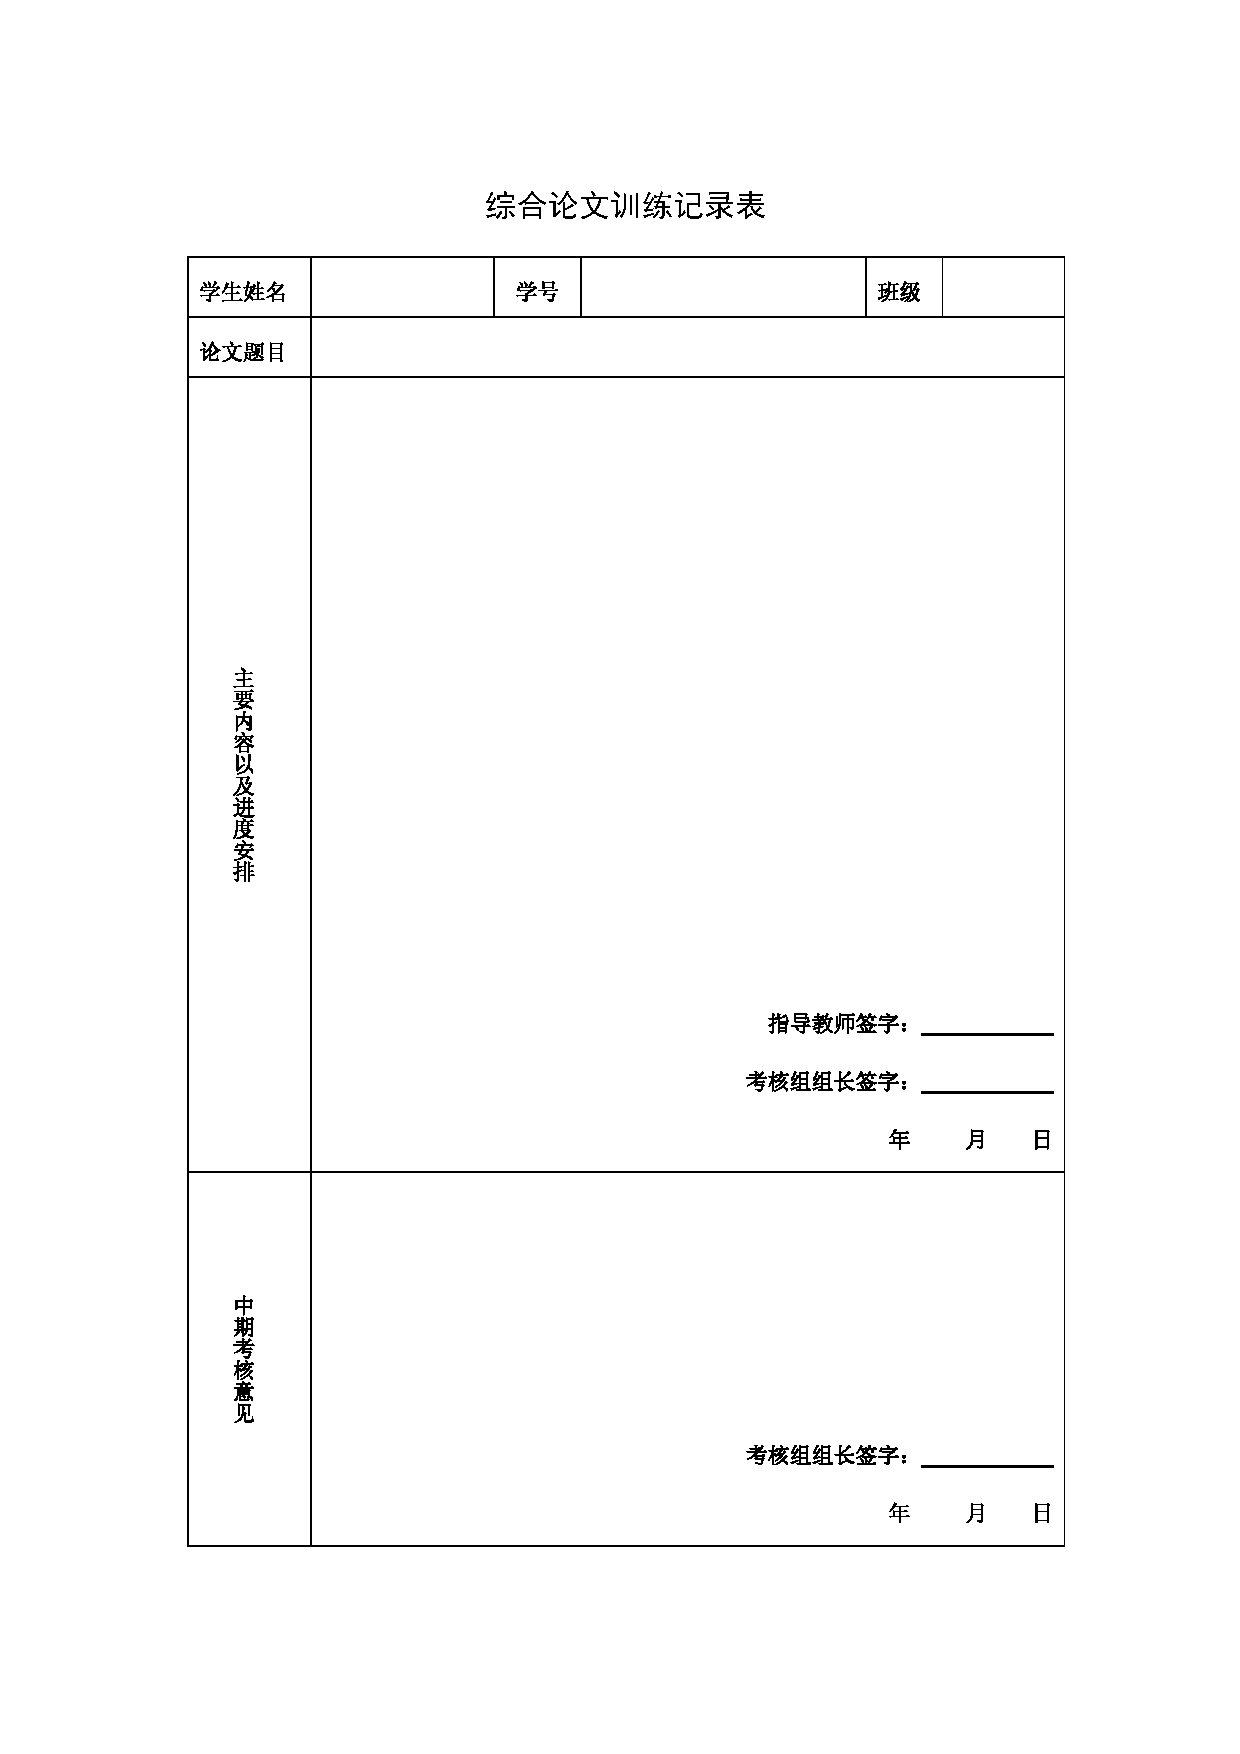
\includepdf[pages=-]{scan-record.pdf}
\end{document}
